\documentclass{article}
\usepackage{nirav-ds203}

\newcommand{\myname}{Nirav Bhattad}
\newcommand{\topicname}{DS203 : Exercise 6}

\begin{document}

\thispagestyle{empty}

\titleBC

\section{Problem 1}

\subsection{Introduction}

This report presents an analysis of the HT R Phase Current dataset. The primary goal is to identify an unstable period within the data and apply various outlier handling techniques, including imputation, trimming, capping, and robust estimation. The findings are illustrated with visualizations, and a statistical comparison of the methods is provided.

\begin{figure}[H]
	\centering
	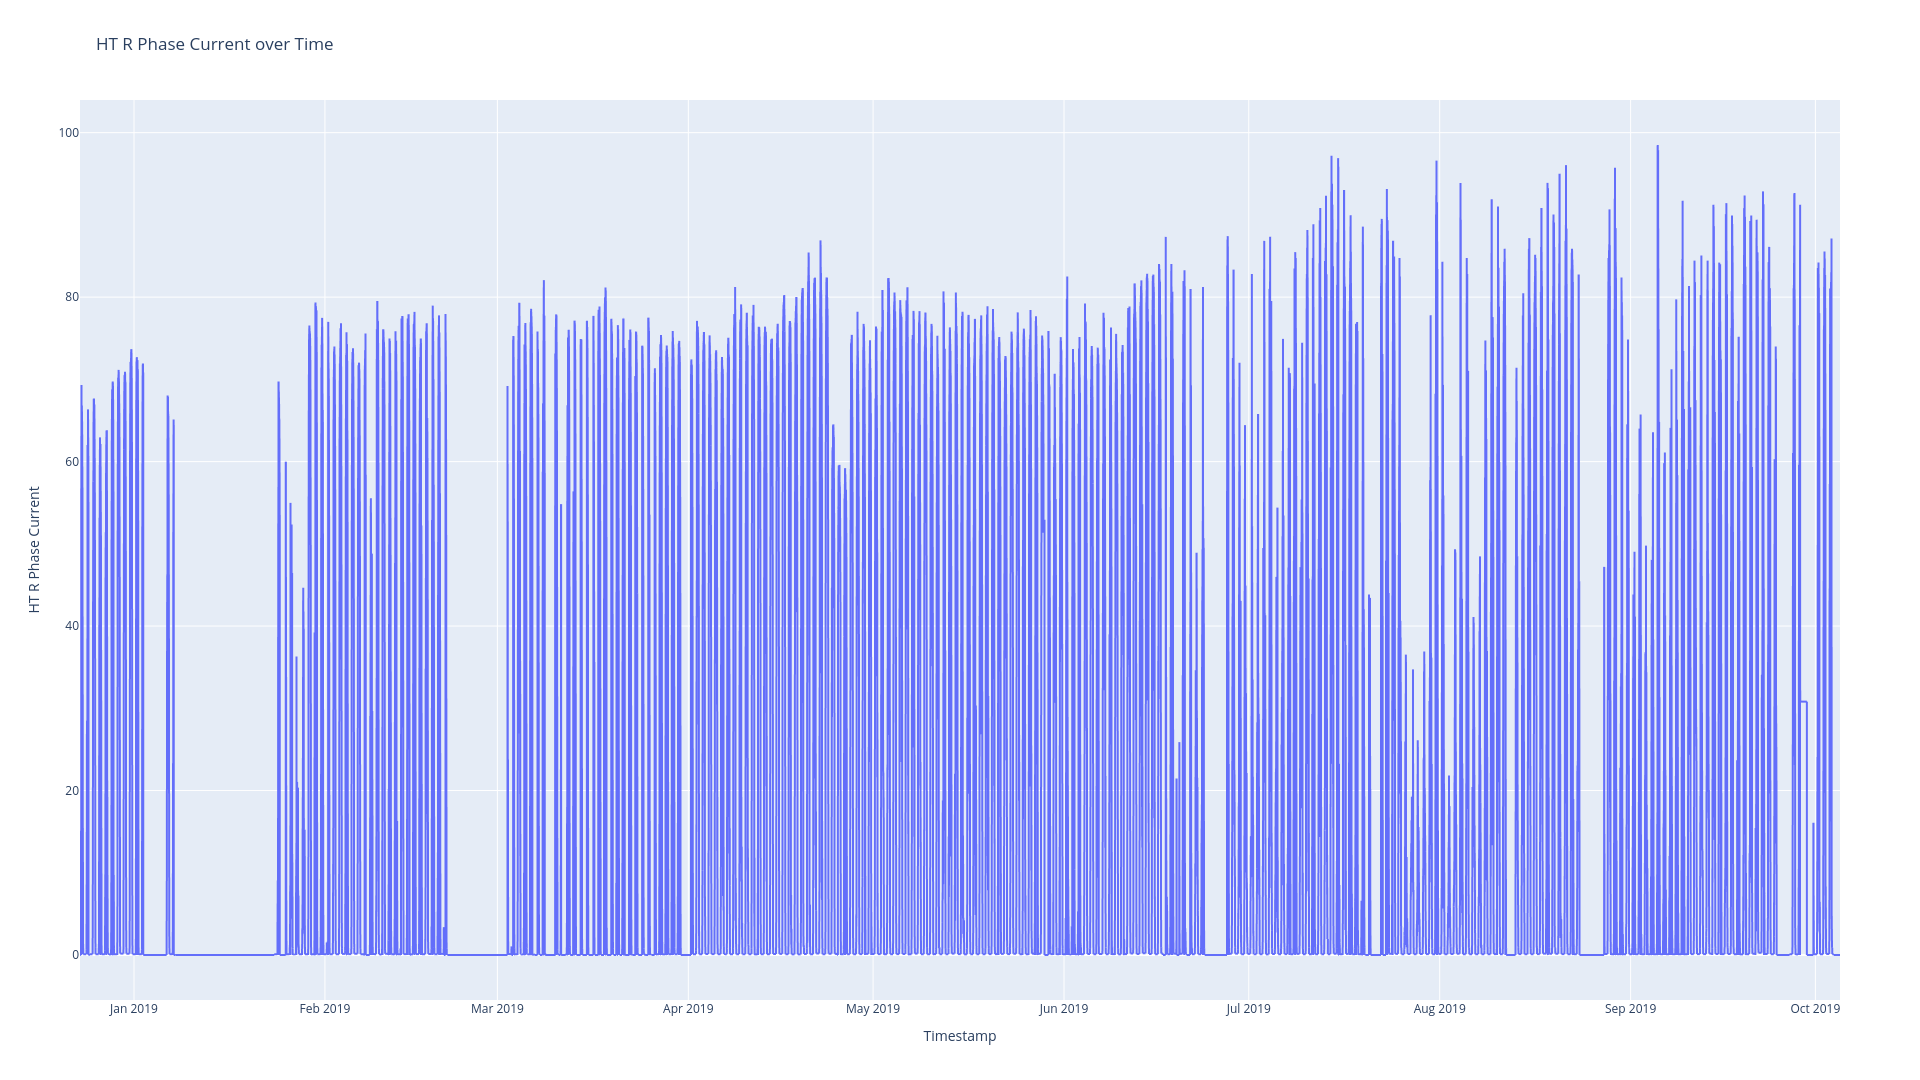
\includegraphics[width=\textwidth]{./Images/ht_r_phase_current.png}
	\caption{HT R Phase Current Dataset}
\end{figure}

\clearpage

\subsection{Data Exploration}

The dataset contains 1,000 records with a mean current of $16.912767$, a standard deviation of $27.174448$, and a range from $0$ to $98.500000$. The data is collected over a period of $9$ Months, with a frequency of $1$ record every $5$ minutes.

% \vspace{2em}

\begin{lstlisting}[language=Python]
import pandas as pd
import numpy as np
import plotly.express as px
import matplotlib.pyplot as plt
from scipy import stats
import os

# Create directory for saving images
if not os.path.exists('Images'):
    os.makedirs('Images')

# Load data from CSV
data = pd.read_csv("e6-htr-current.csv", parse_dates=['Timestamp'], dayfirst=True)

# Part A: Perform EDA
print(data.describe())

# Plot the current over time using Plotly
fig = px.line(data, x='Timestamp', y='HT R Phase Current', title='HT R Phase Current over Time')
fig.write_image("Images/ht_r_phase_current.png", scale=1, width=1920, height=1080, format='png')
fig.show()

# Part B: Identify a 2-week unstable period
unstable_period = data[(data['Timestamp'] >= '2019-07-30') & (data['Timestamp'] <= '2019-08-14')].copy()

# Plot the unstable period
plt.figure(figsize=(16, 10))
plt.plot(unstable_period['Timestamp'], unstable_period['HT R Phase Current'], color='blue')
plt.title('HT R Phase Current - Unstable Period')
plt.xlabel('Timestamp')
plt.ylabel('Current')
plt.savefig('Images/unstable_period.png', dpi=300)
plt.show()
\end{lstlisting}

Using the plot above, we can identify an unstable period between July 30, 2019, and August 14, 2019. This period will be used to evaluate the outlier handling techniques.

\begin{figure}[H]
	\centering
	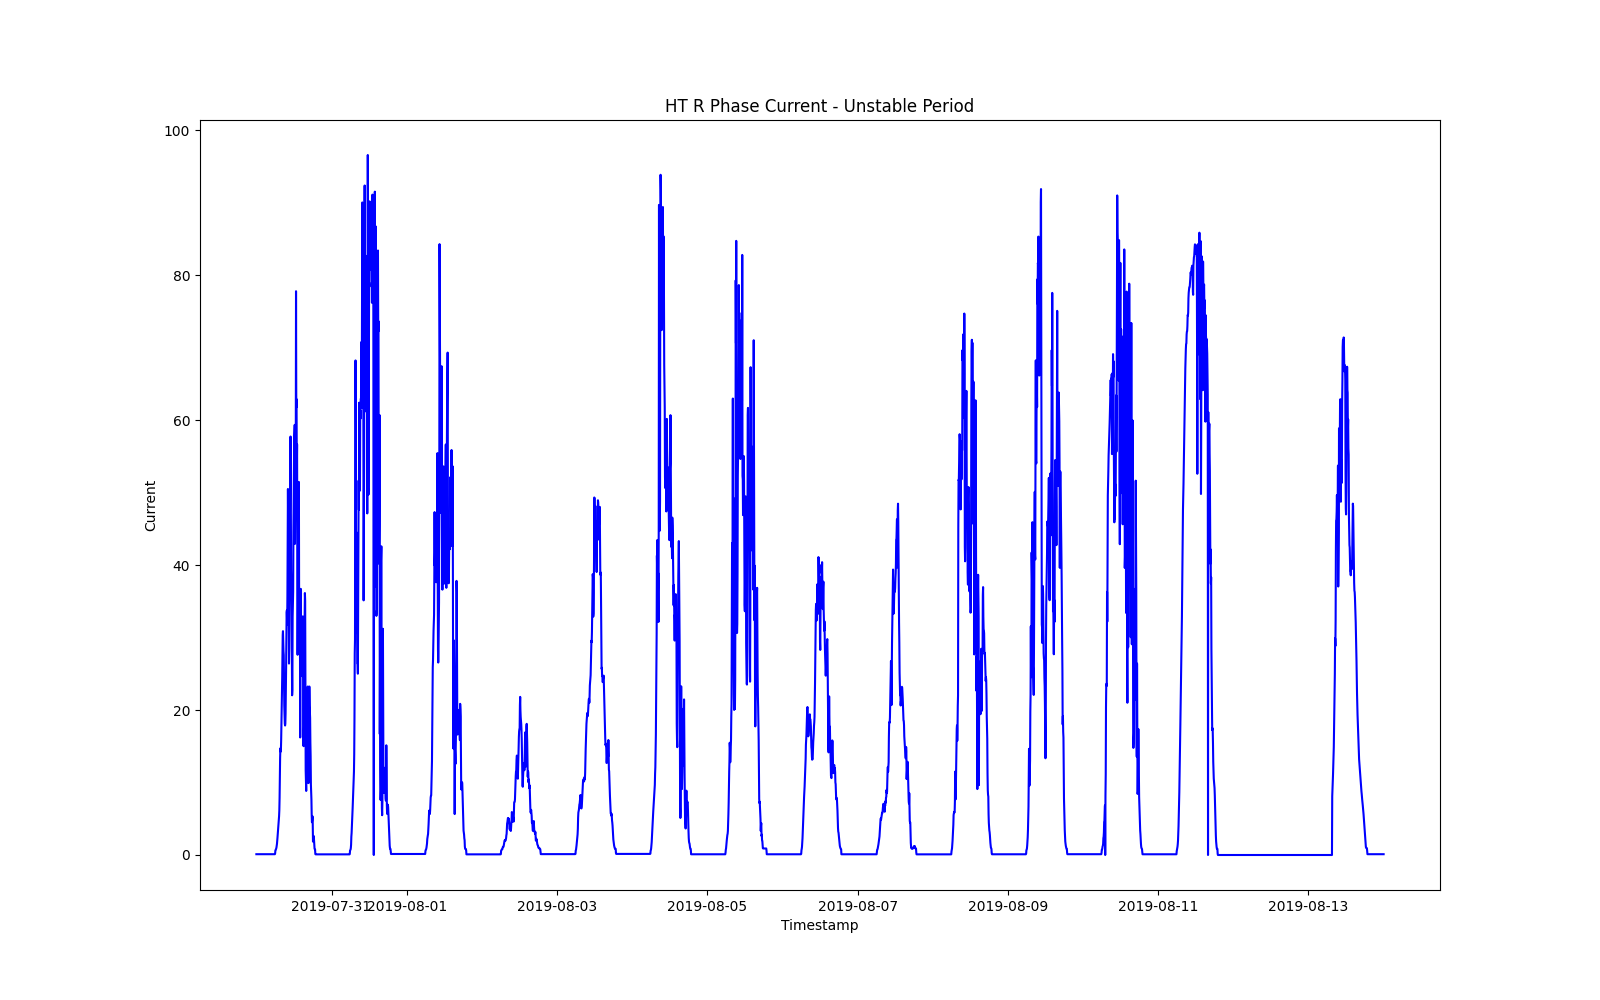
\includegraphics[width=0.65\textwidth]{./Images/unstable_period.png}
	\caption{HT R Phase Current - Unstable Period}
\end{figure}

\subsection{Removing outliers, smoothening, and imputing missing data}

Here we apply four outlier handling techniques to the unstable period: imputation, trimming, capping, and robust estimation. The results are visualized to compare the effectiveness of each method.

\begin{lstlisting}[language=Python, gobble=0]
# Method 1: Imputation (Replacing outlier values with the mean)
mean_value = unstable_period['HT R Phase Current'].mean()
median_value = unstable_period['HT R Phase Current'].median()
unstable_period['Current_Imputed_Mean'] = unstable_period['HT R Phase Current'].copy()
unstable_period.loc[(unstable_period['HT R Phase Current'] > unstable_period['HT R Phase Current'].quantile(0.95)) | (unstable_period['HT R Phase Current'] < unstable_period['HT R Phase Current'].quantile(0.05)), 'Current_Imputed_Mean'] = mean_value

unstable_period['Current_Imputed_Median'] = unstable_period['HT R Phase Current'].copy()
unstable_period.loc[(unstable_period['HT R Phase Current'] > unstable_period['HT R Phase Current'].quantile(0.95)) | (unstable_period['HT R Phase Current'] < unstable_period['HT R Phase Current'].quantile(0.05)), 'Current_Imputed_Median'] = median_value

# Method 2: Trimming (Removing outliers)
q_low = unstable_period['HT R Phase Current'].quantile(0.1)
q_high = unstable_period['HT R Phase Current'].quantile(0.9)
unstable_period_trimmed = unstable_period[(unstable_period['HT R Phase Current'] >= q_low) & (unstable_period['HT R Phase Current'] <= q_high)]

# Method 3: Capping (Setting a cap on the maximum and minimum values)
max_value = unstable_period['HT R Phase Current'].quantile(0.95)
min_value = unstable_period['HT R Phase Current'].quantile(0.05)
unstable_period['Current_Capped'] = unstable_period['HT R Phase Current'].copy()
unstable_period['Current_Capped'] = np.where(unstable_period['Current_Capped'] > max_value, max_value, unstable_period['Current_Capped'])
unstable_period['Current_Capped'] = np.where(unstable_period['Current_Capped'] < min_value, min_value, unstable_period['Current_Capped'])

# Method 4: Robust Estimation (Using RANSAC regression)
from sklearn.linear_model import RANSACRegressor, LinearRegression

# Prepare the data for RANSAC
X = unstable_period['Timestamp'].map(pd.Timestamp.timestamp).values.reshape(-1, 1)  # Convert datetime to timestamp
y = unstable_period['HT R Phase Current'].values

# Fit RANSAC
model = RANSACRegressor(LinearRegression()).fit(X, y)
unstable_period['Current_Robust'] = model.predict(X)
\end{lstlisting}

I have used the following techniques to handle the outliers:

\begin{itemize}
	\item \textbf{Imputation:} Replacing outlier values with the mean or median of the data.
	\item \textbf{Trimming:} Removing outliers from the dataset.
	\item \textbf{Capping:} Setting a cap on the maximum and minimum values.
	\item \textbf{Robust Estimation:} Using RANSAC regression to estimate the data without outliers.
\end{itemize}


\begin{figure}[H]
	\centering
	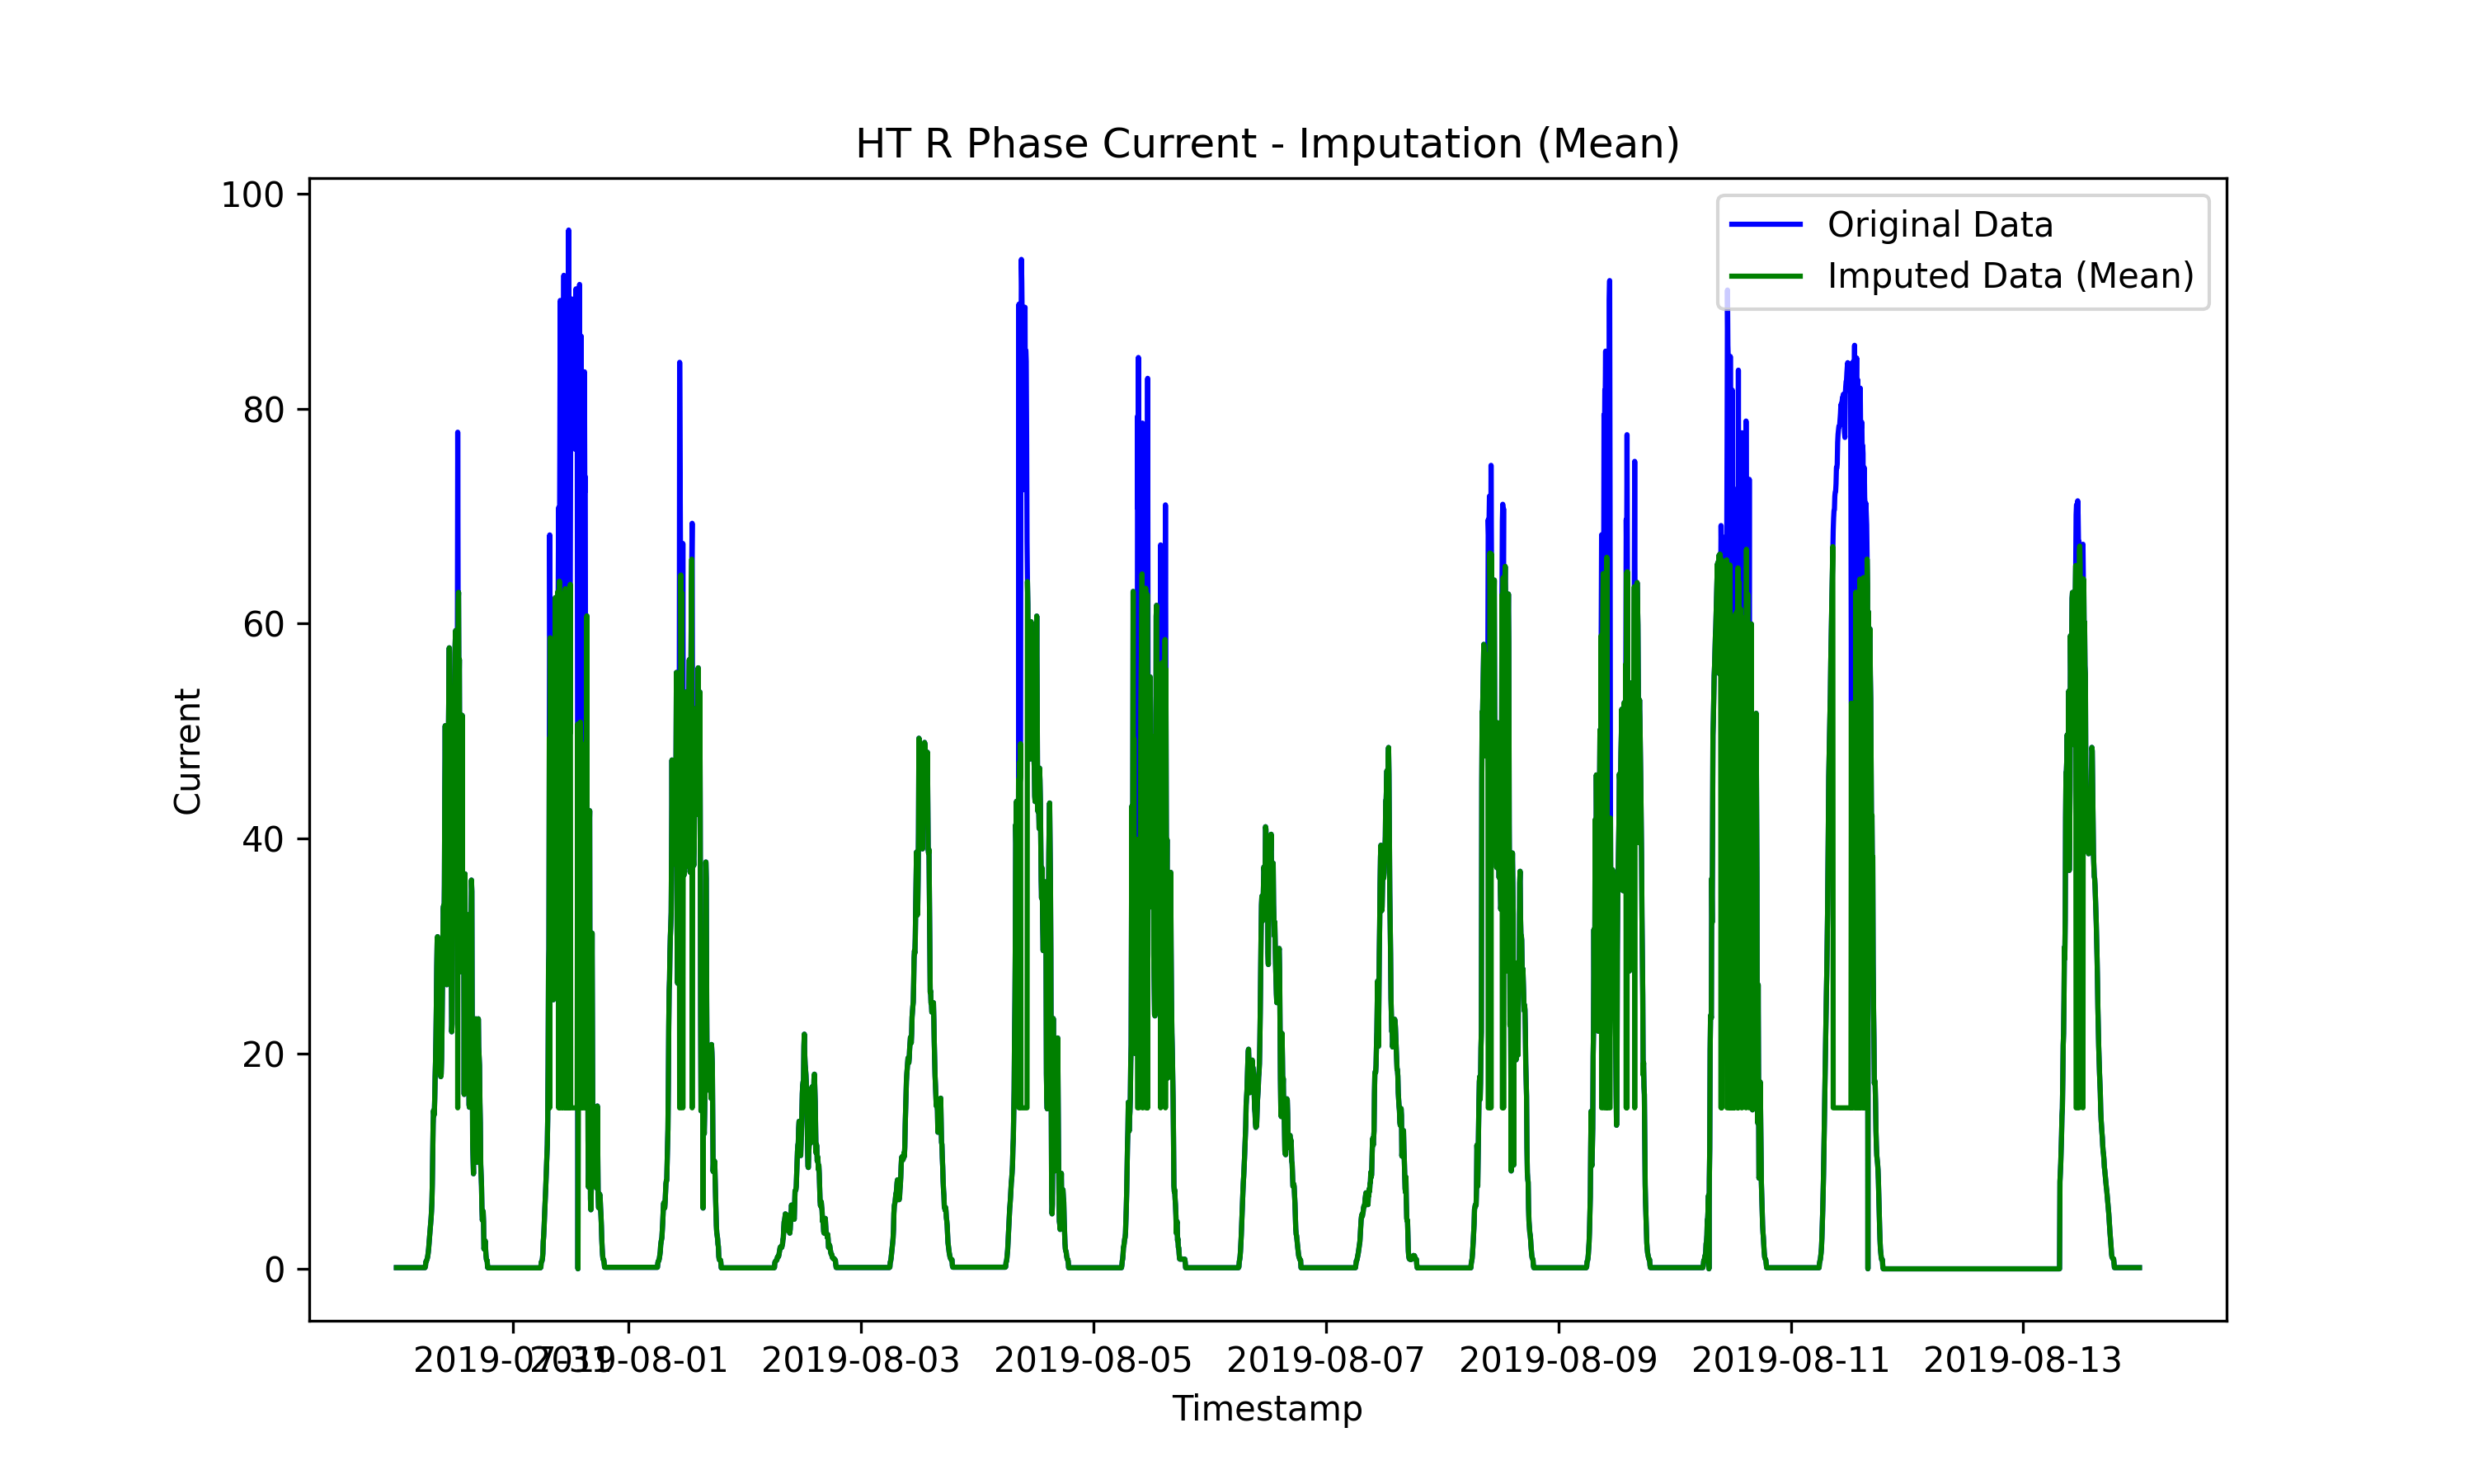
\includegraphics[width=0.9\textwidth]{./Images/imputed_mean_data.png}
	\caption{Imputed Mean Data}
\end{figure}

\begin{figure}[H]
	\centering
	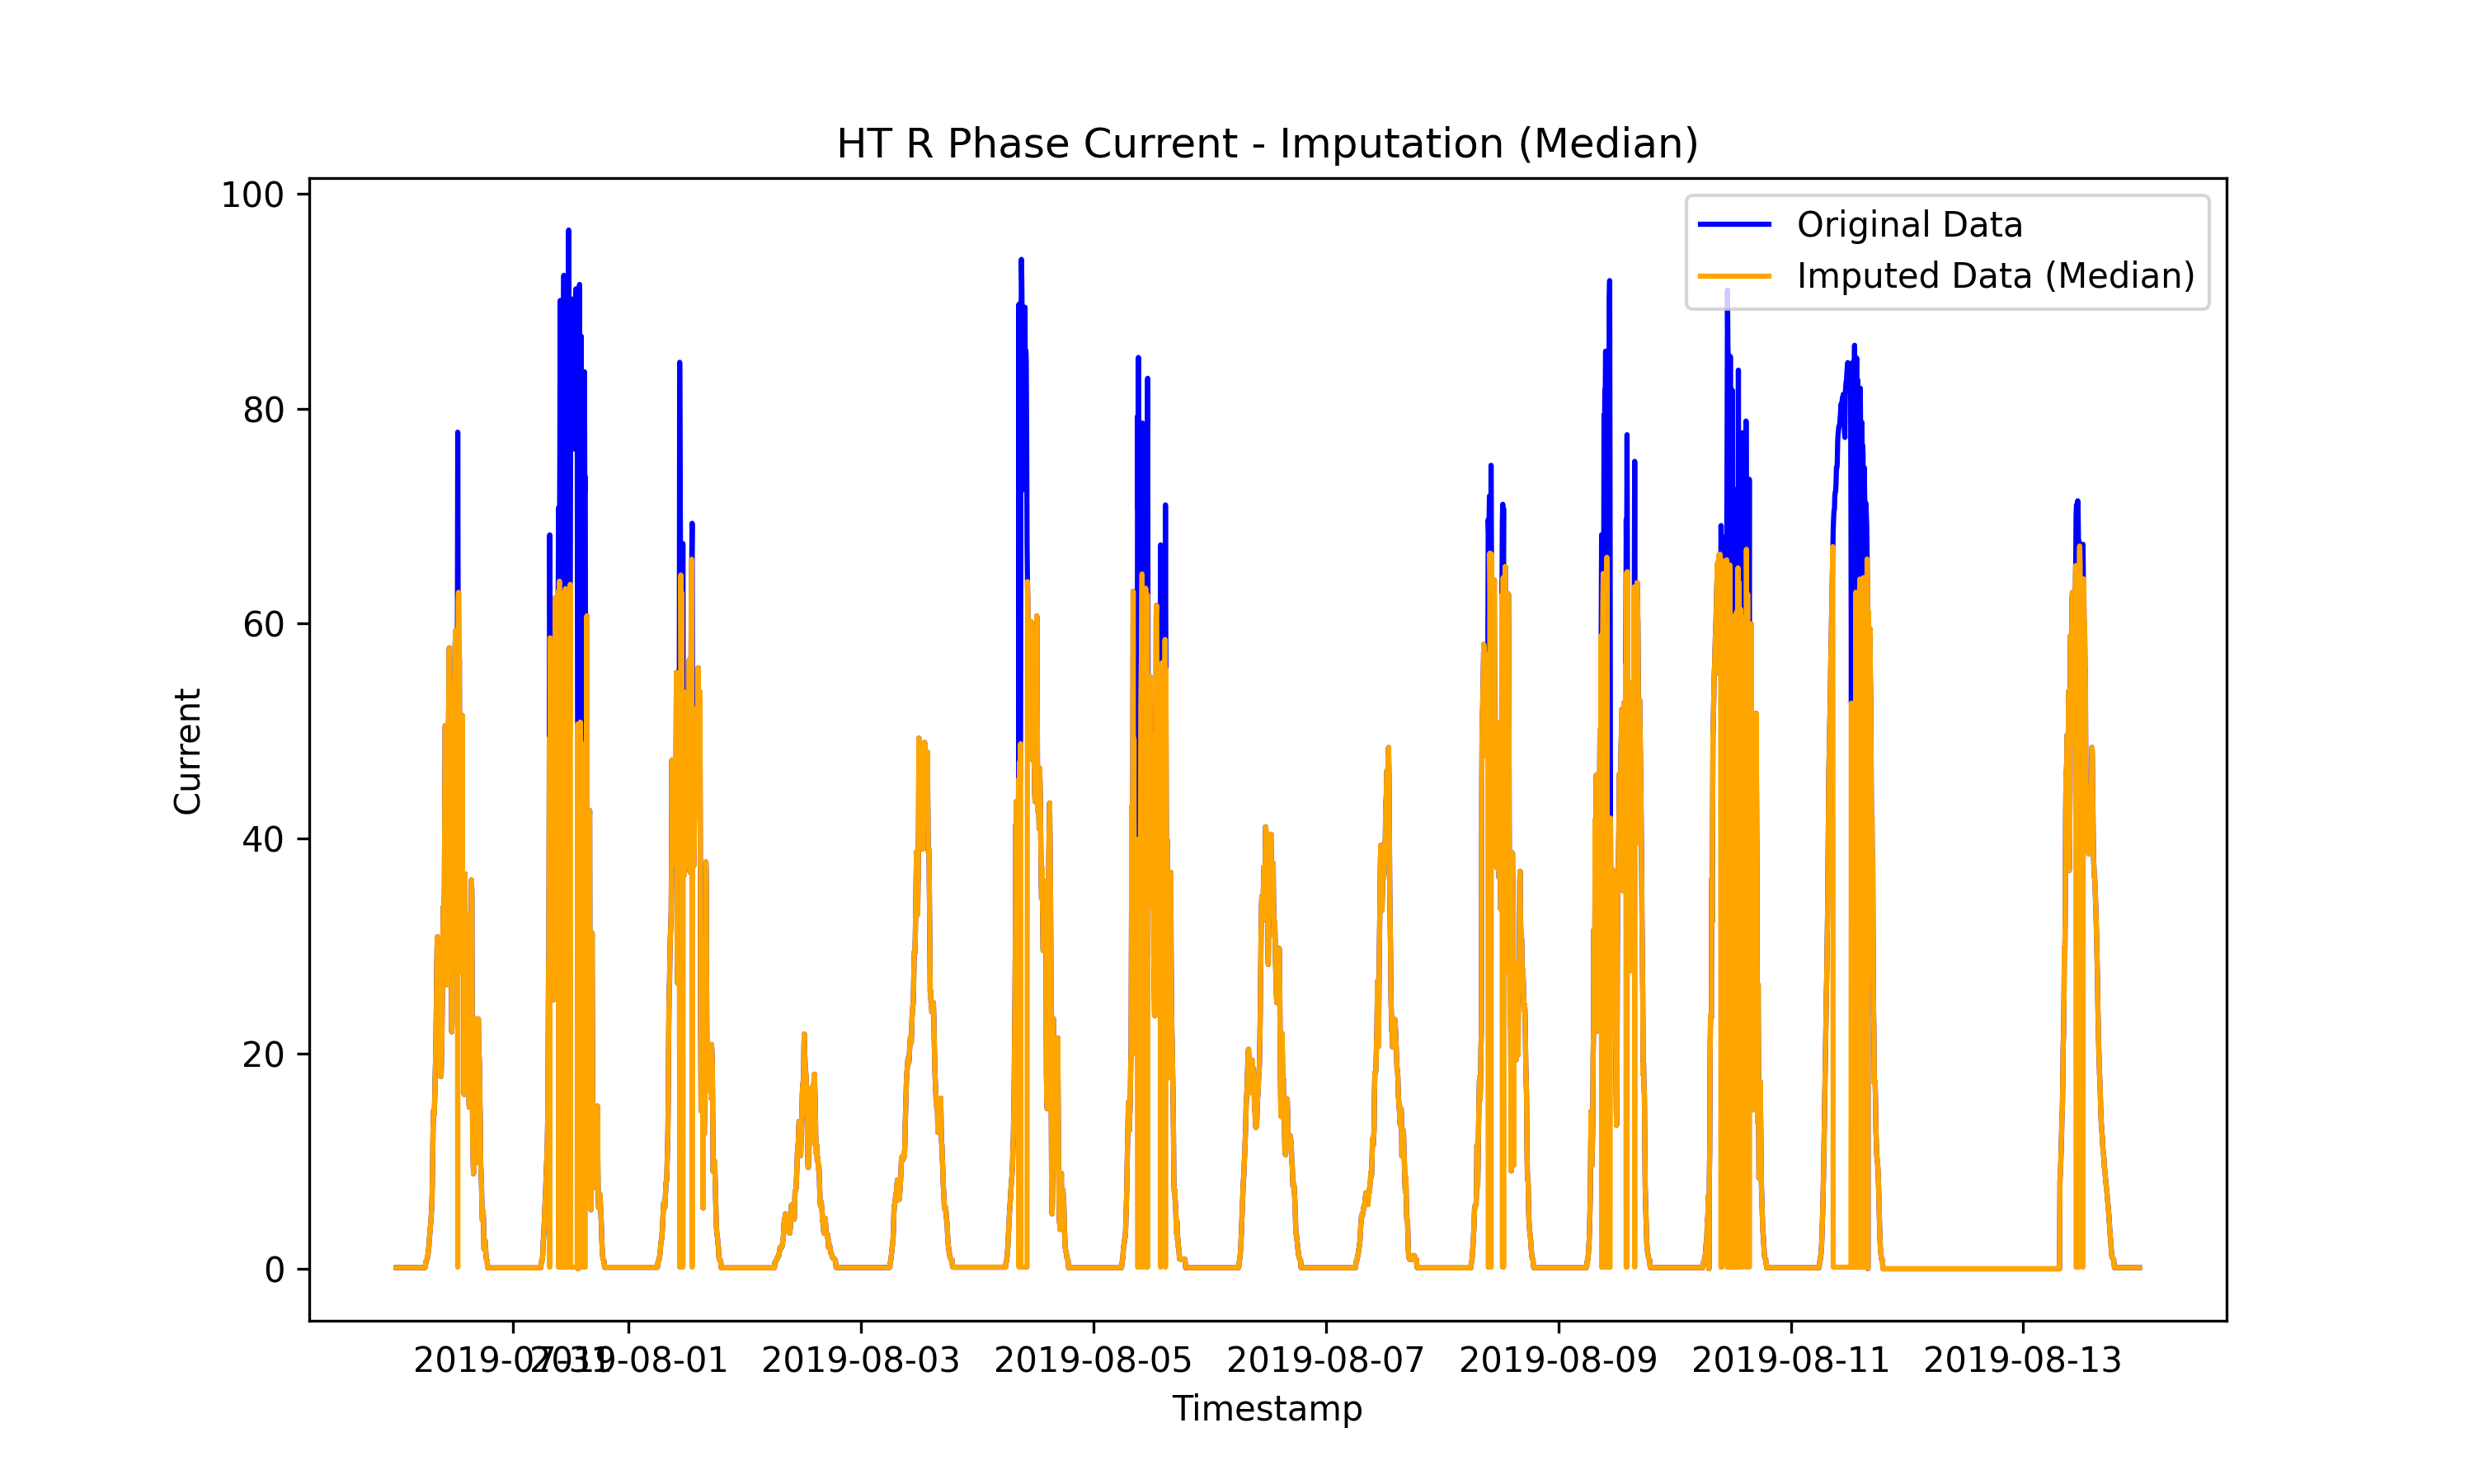
\includegraphics[width=0.9\textwidth]{./Images/imputed_median_data.png}
	\caption{Imputed Median Data}
\end{figure}

\begin{figure}[H]
	\centering
	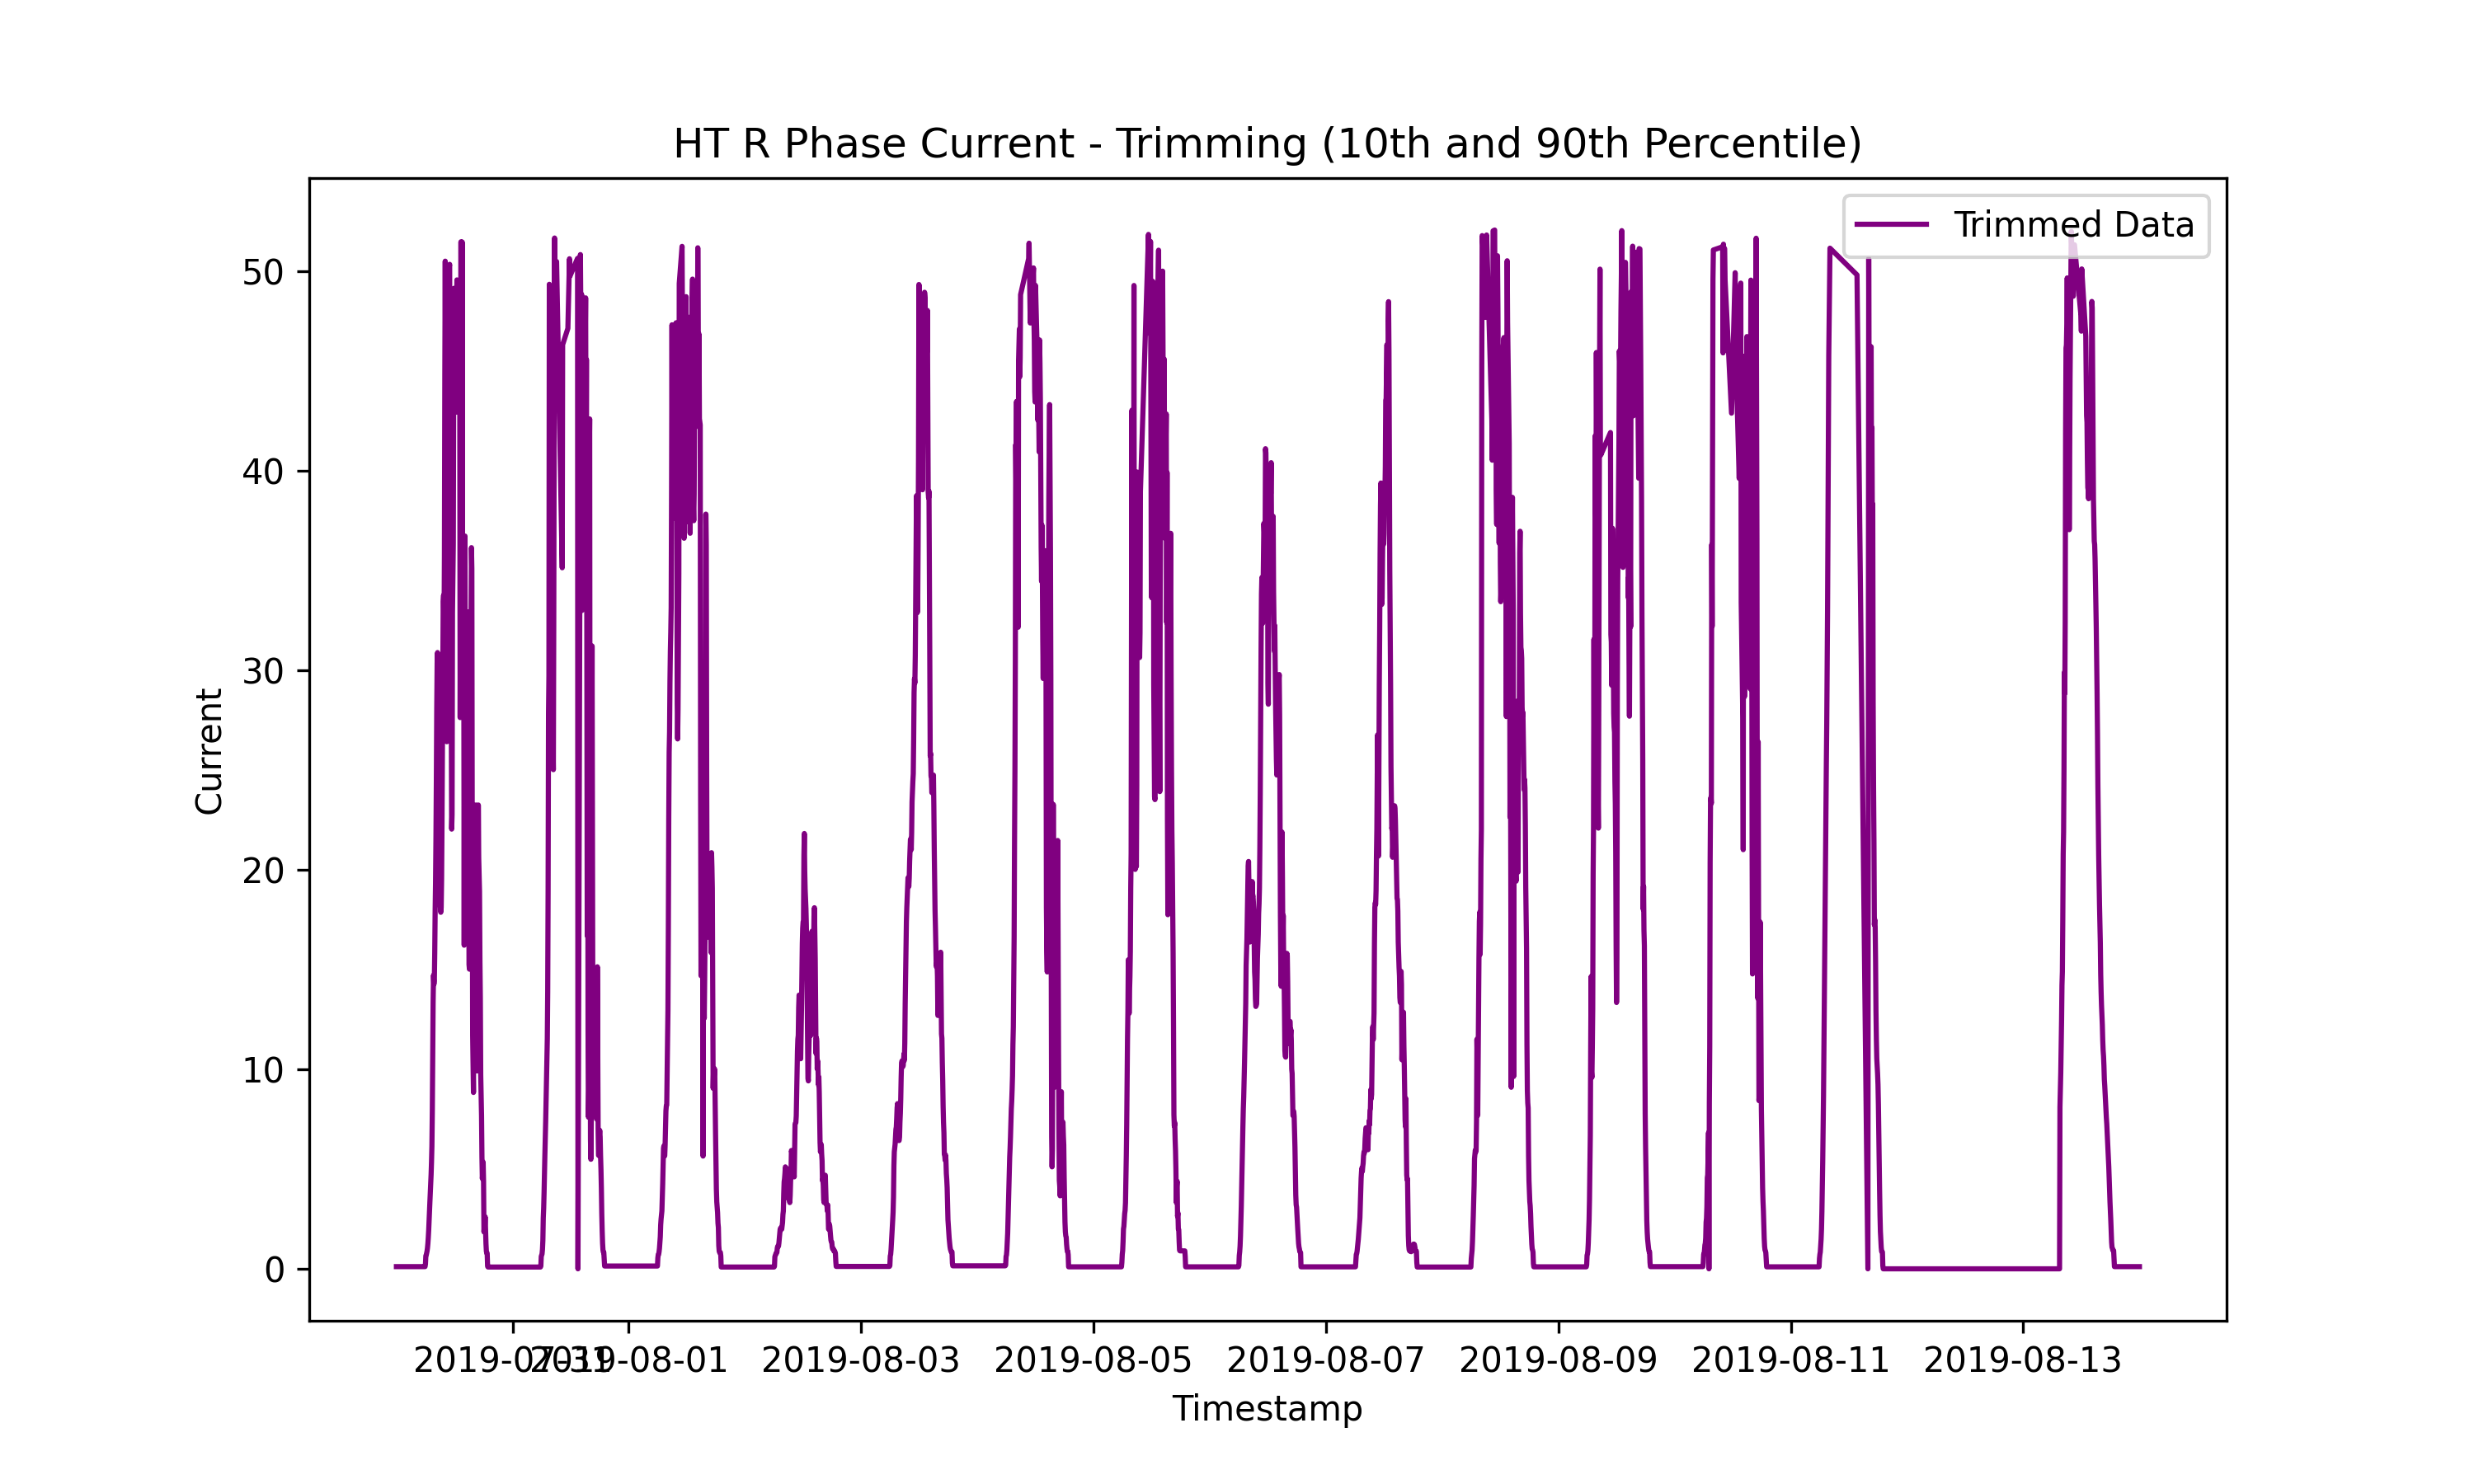
\includegraphics[width=0.9\textwidth]{./Images/trimmed_data.png}
	\caption{Trimmed Data}
\end{figure}

\begin{figure}[H]
	\centering
	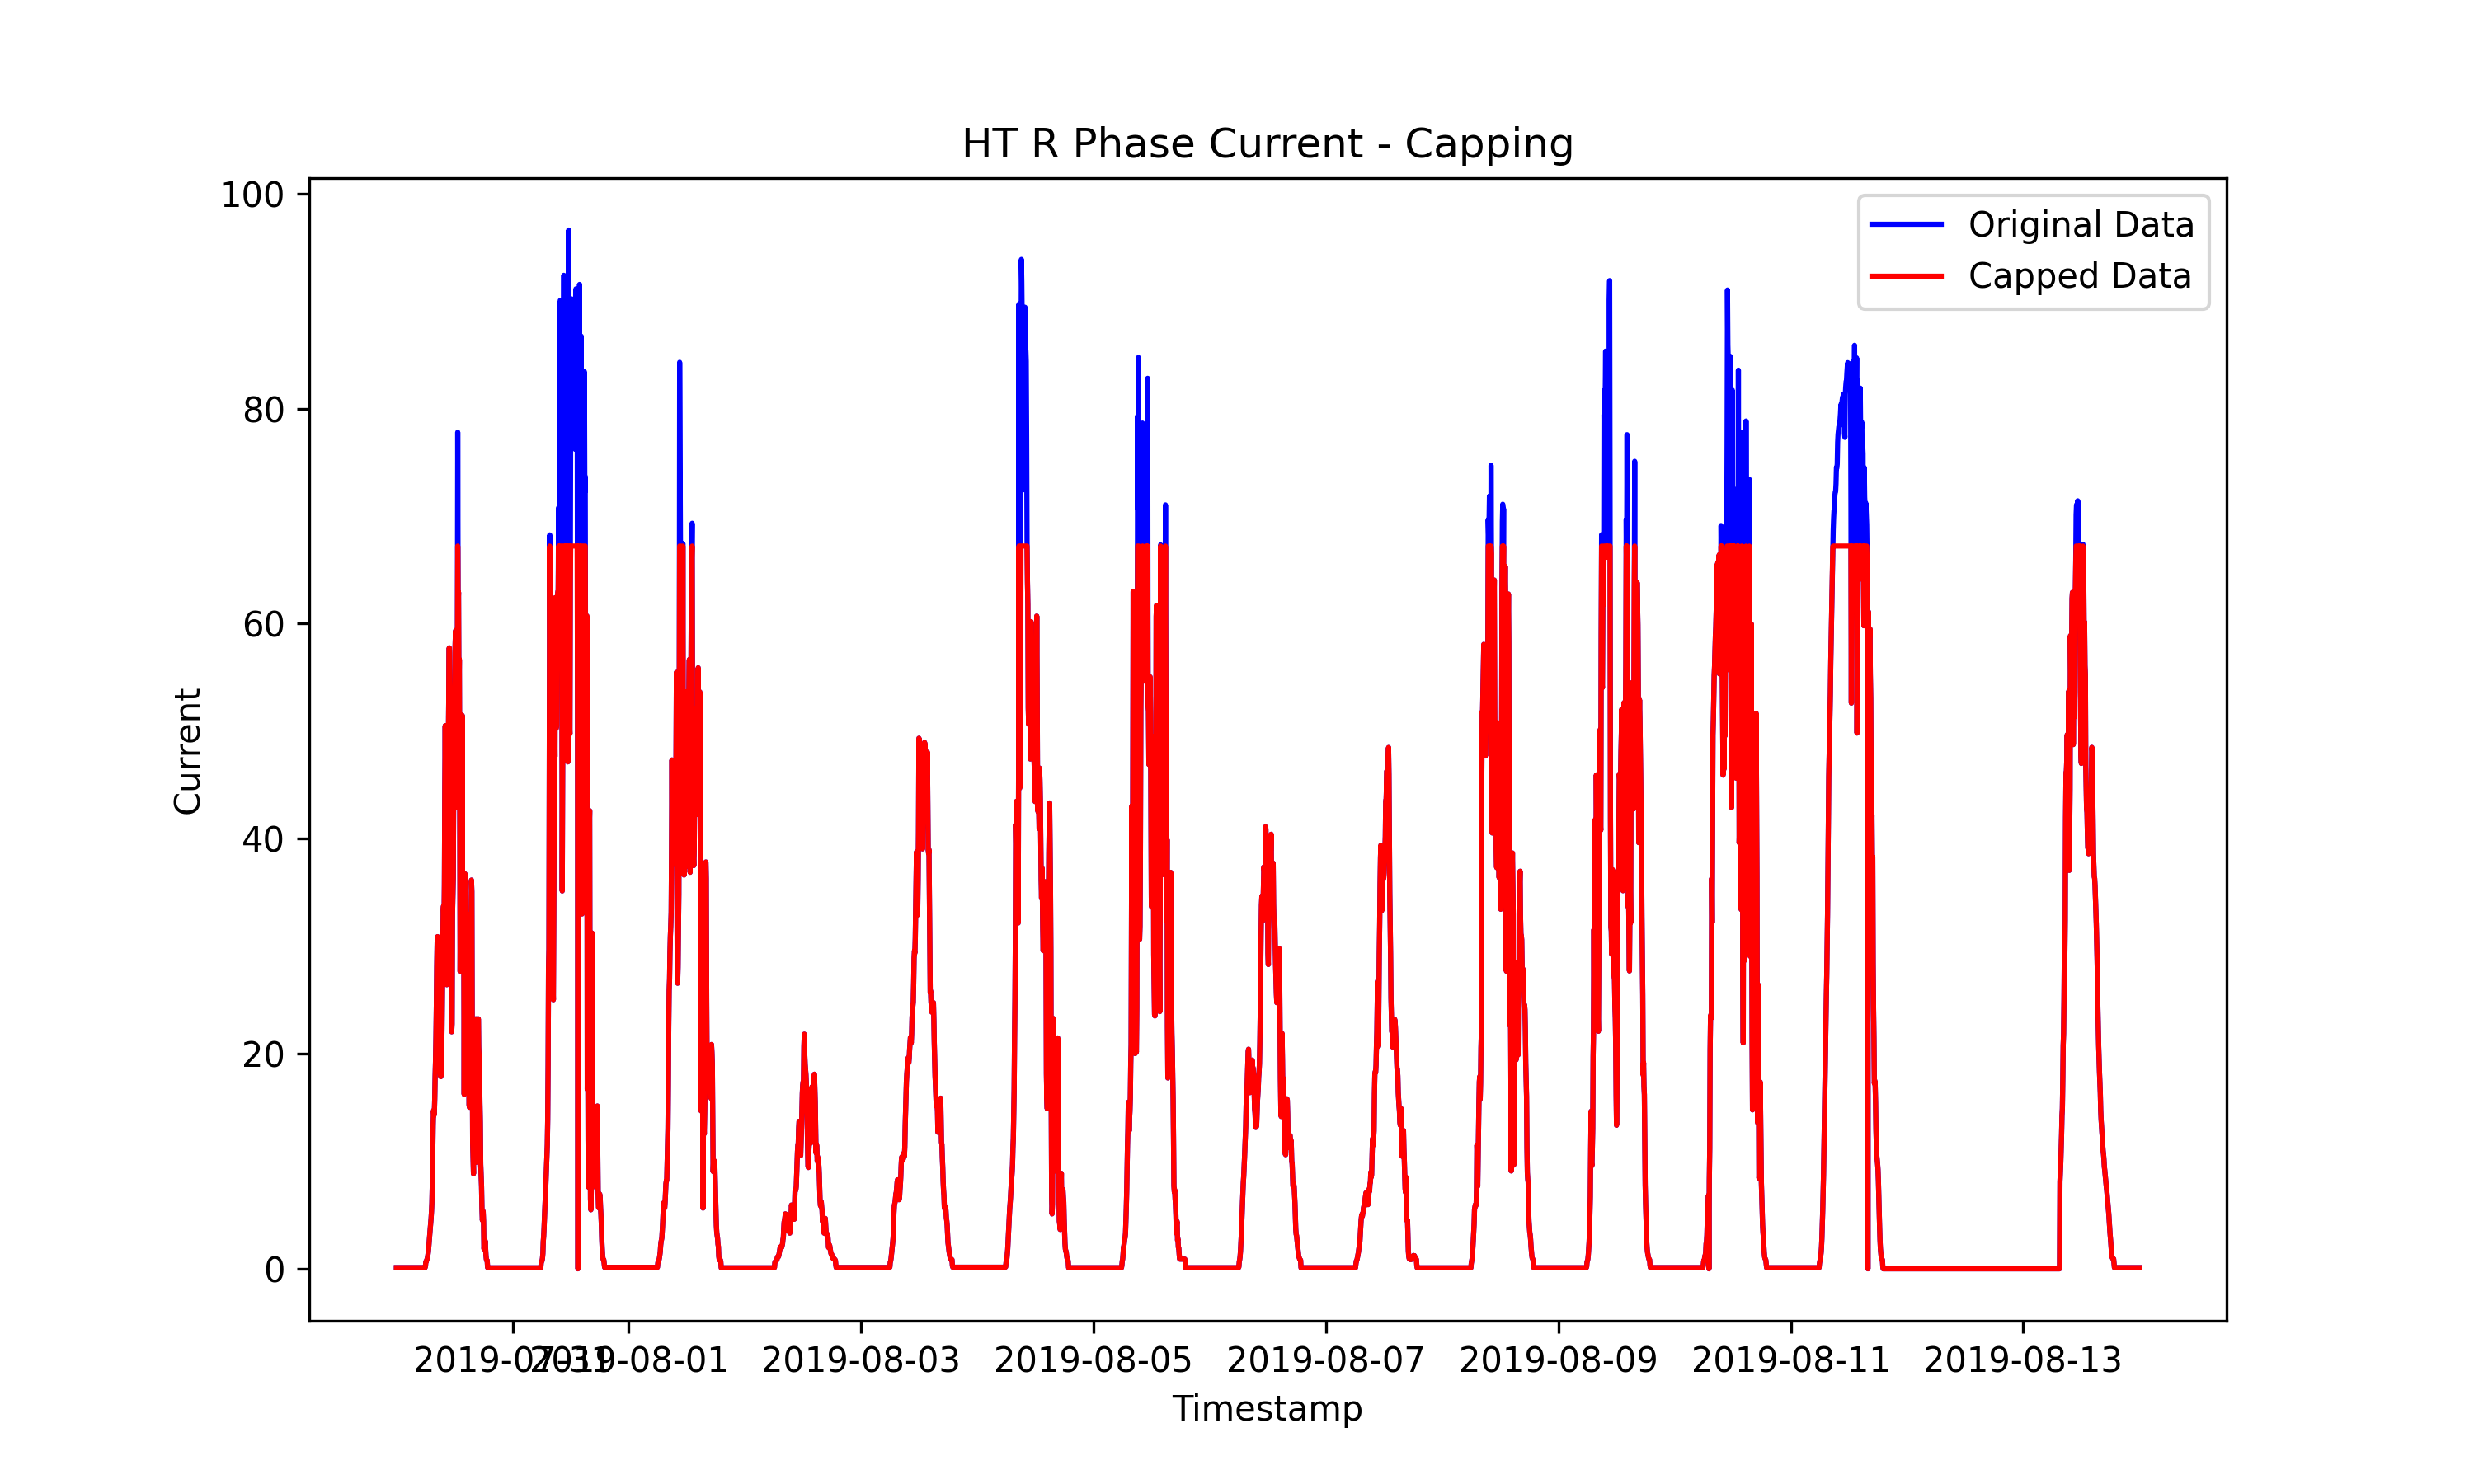
\includegraphics[width=0.9\textwidth]{./Images/capped_data.png}
	\caption{Capped Data}
\end{figure}

\begin{figure}[H]
	\centering
	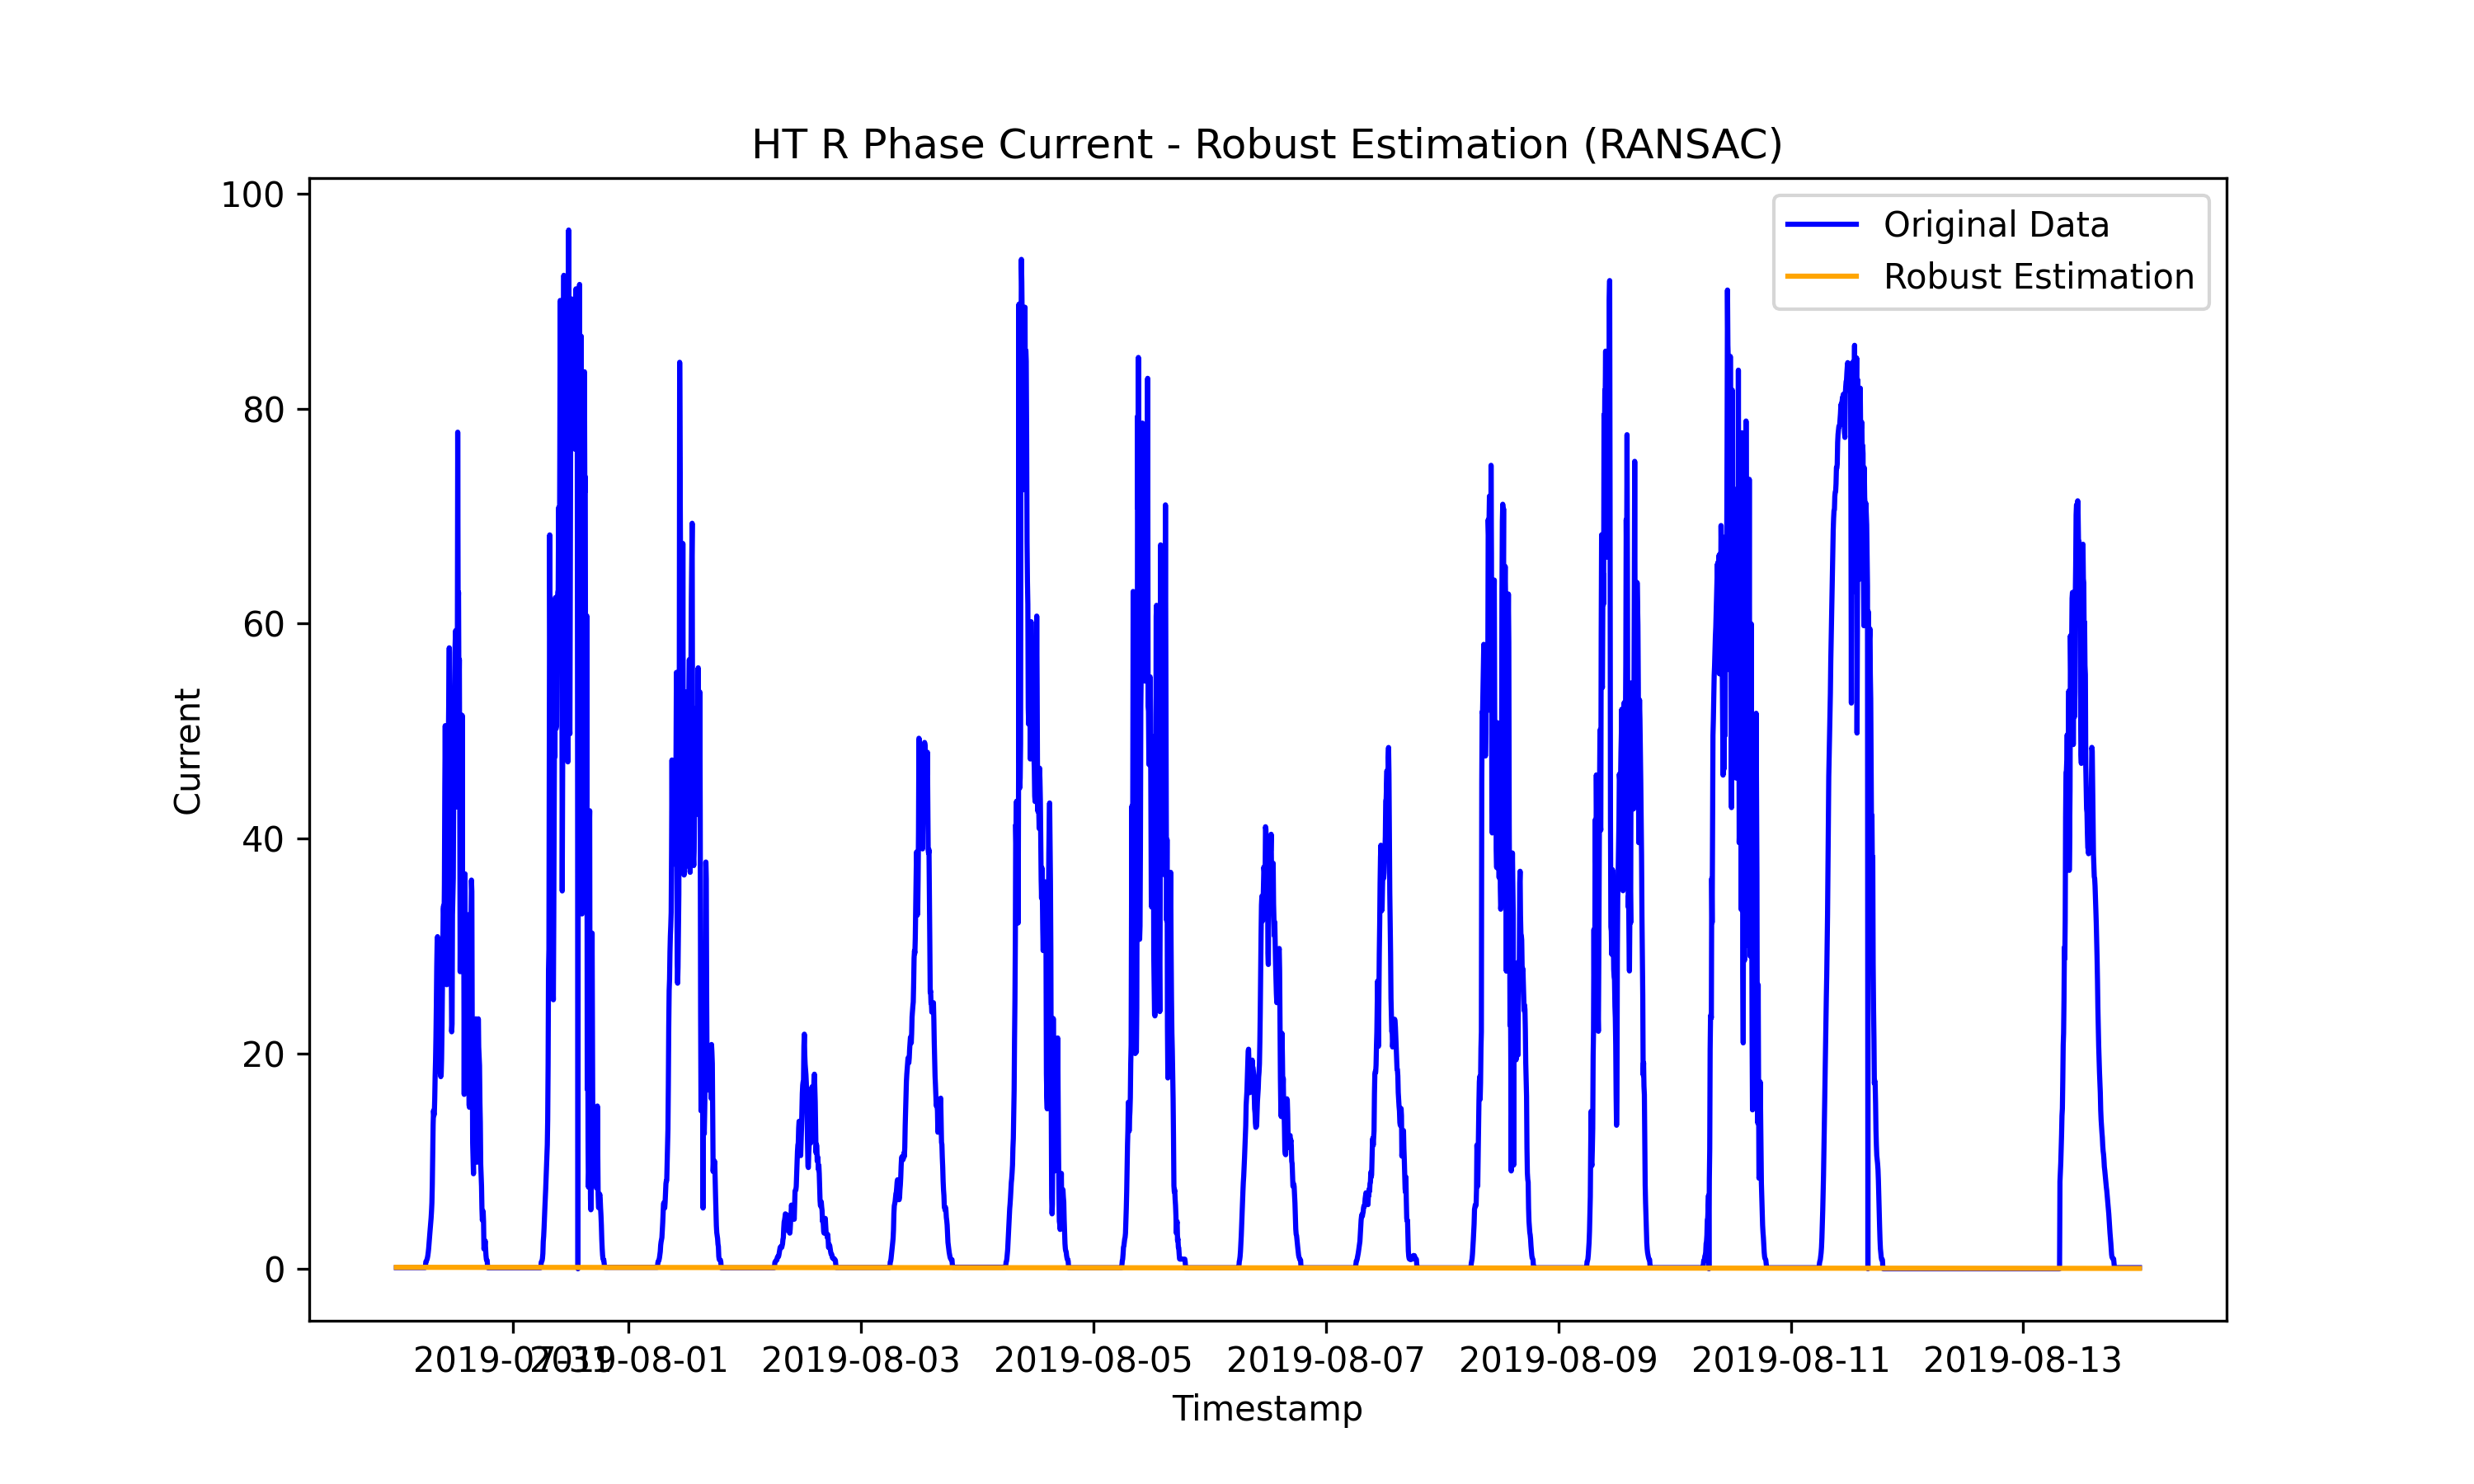
\includegraphics[width=0.9\textwidth]{./Images/robust_estimation_data.png}
	\caption{Robust Data}
\end{figure}

% Outlies Handing comparison image
\begin{figure}[H]
	\centering
	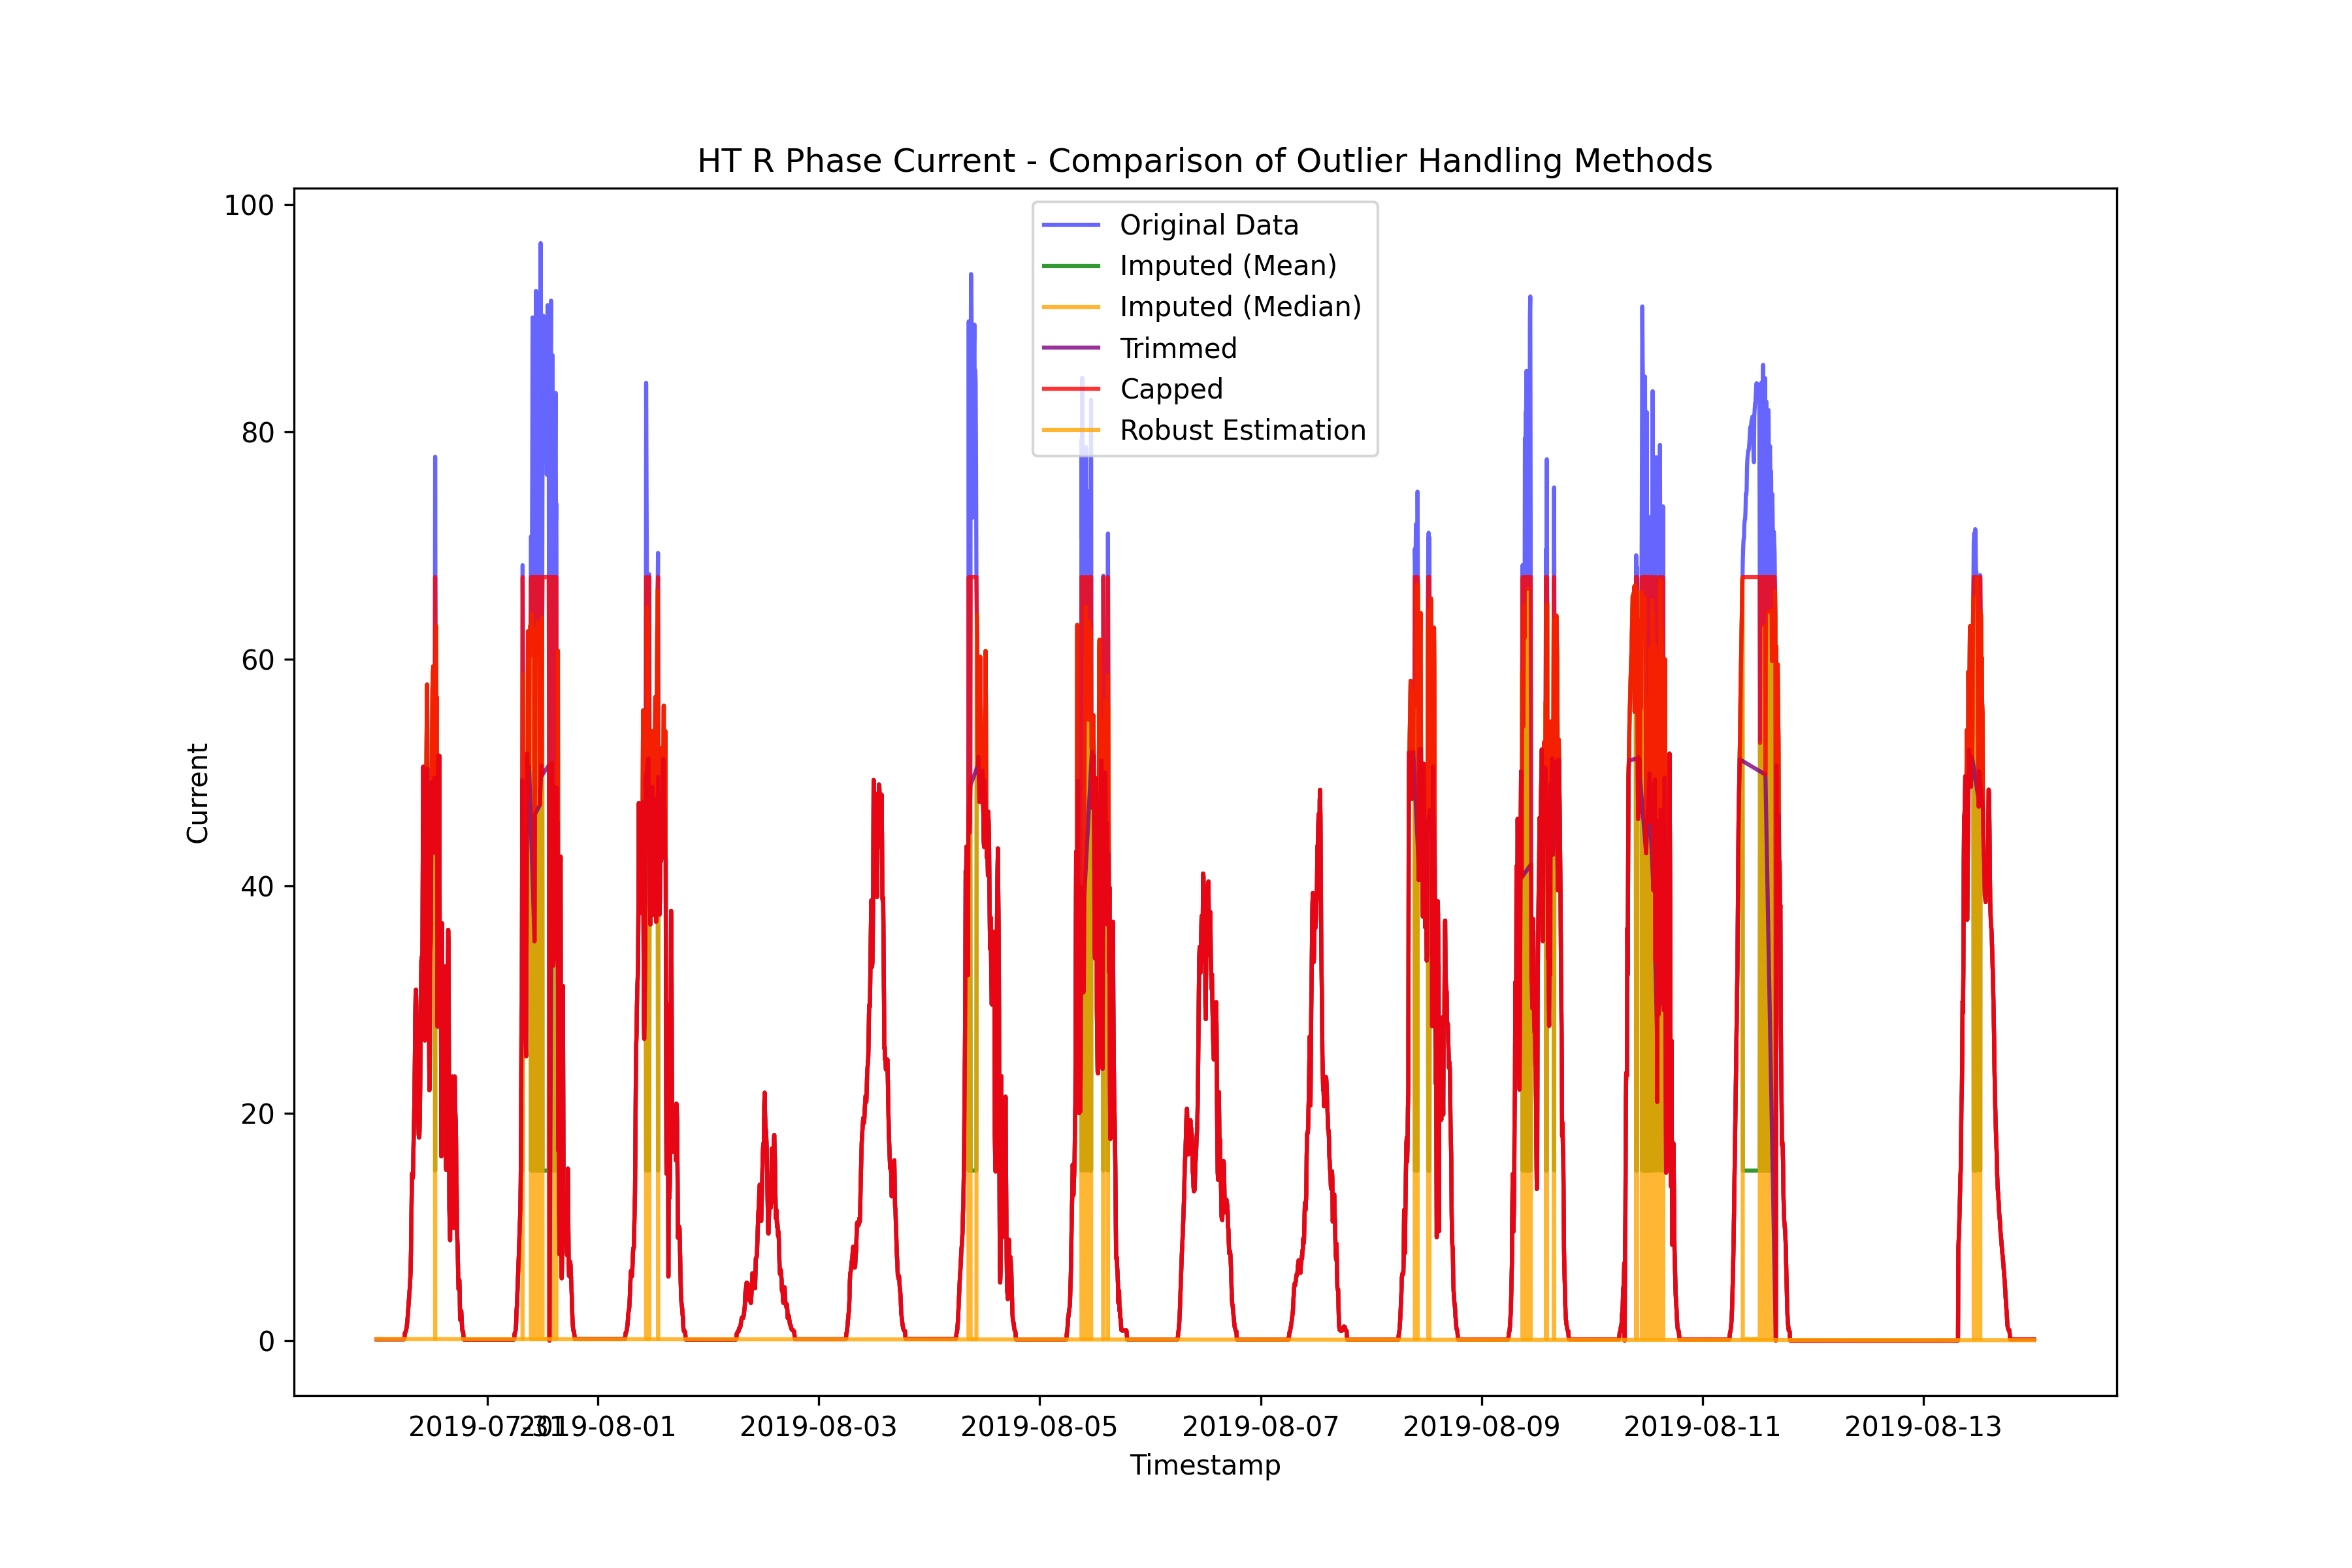
\includegraphics[width=0.9\textwidth]{./Images/outlier_handling_comparison.png}
	\caption{Outlier Handling Comparison}
\end{figure}



\clearpage
\section{Problem 2}

\subsection{Introduction}

This report presents a comprehensive data analysis workflow applied to the dataset \texttt{e6-Run2-June22-subset-100-cols.csv}. The main objectives include data cleaning, outlier detection, normalization, correlation analysis, multicollinearity assessment, and Principal Component Analysis (PCA).

\subsection{Methodology}

\subsubsection{Data Loading and Initial Exploration}
The data was loaded using the \texttt{pandas} library. Initial exploration was performed to understand the structure and quality of the data.

\begin{lstlisting}[language=Python]
import pandas as pd
import numpy as np
import seaborn as sns
import matplotlib.pyplot as plt

df = pd.read_csv('e6-Run2-June22-subset-100-cols.csv')
print(df.head(10))
print(df.describe())
print(df.isnull().sum())
\end{lstlisting}

\subsubsection{Data Cleaning}
Data cleaning involved the following steps:

\begin{itemize}
    \item **Column Retention:** Columns with low variance were dropped based on a variance threshold of 0.05.
    \item **Handling Missing Values:** Missing values were replaced with the mean of each column.
    \item **Outlier Detection:** Outliers were detected using the Interquartile Range (IQR) method, and appropriate action was taken.
\end{itemize}

\begin{lstlisting}[language=Python]
# Step 1: Replace non-numeric values
df.replace('#REF!', np.nan, inplace=True)

# Step 2: Drop low variance columns
variances = df.var()
low_variance_columns = variances[variances < 0.05].index
df.drop(columns=low_variance_columns, inplace=True)

# Step 3: Handle missing values
df.fillna(df.mean(), inplace=True)

# Step 4: Outlier detection using IQR
Q1 = df.quantile(0.25)
Q3 = df.quantile(0.75)
IQR = Q3 - Q1
outlier_condition = (df < (Q1 - 1.5 * IQR)) | (df > (Q3 + 1.5 * IQR))
df = df[~outlier_condition.any(axis=1)]
\end{lstlisting}

\subsubsection{Normalization}
Standardization was performed on the numeric columns to prepare the data for PCA.

\begin{lstlisting}[language=Python]
from sklearn.preprocessing import StandardScaler
scaler = StandardScaler()
df_scaled = pd.DataFrame(scaler.fit_transform(df), columns=df.columns)
\end{lstlisting}

\subsubsection{Correlation Analysis}
A correlation matrix was computed and visualized to identify highly correlated features.

\begin{lstlisting}[language=Python]
corr_matrix = df_scaled.corr()
plt.figure(figsize=(12, 10))
sns.heatmap(corr_matrix, annot=True, fmt=".2f", cmap='RdBu_r', square=True)
plt.title("Correlation Heatmap")
plt.show()
\end{lstlisting}

\begin{figure}[H]
    \centering
    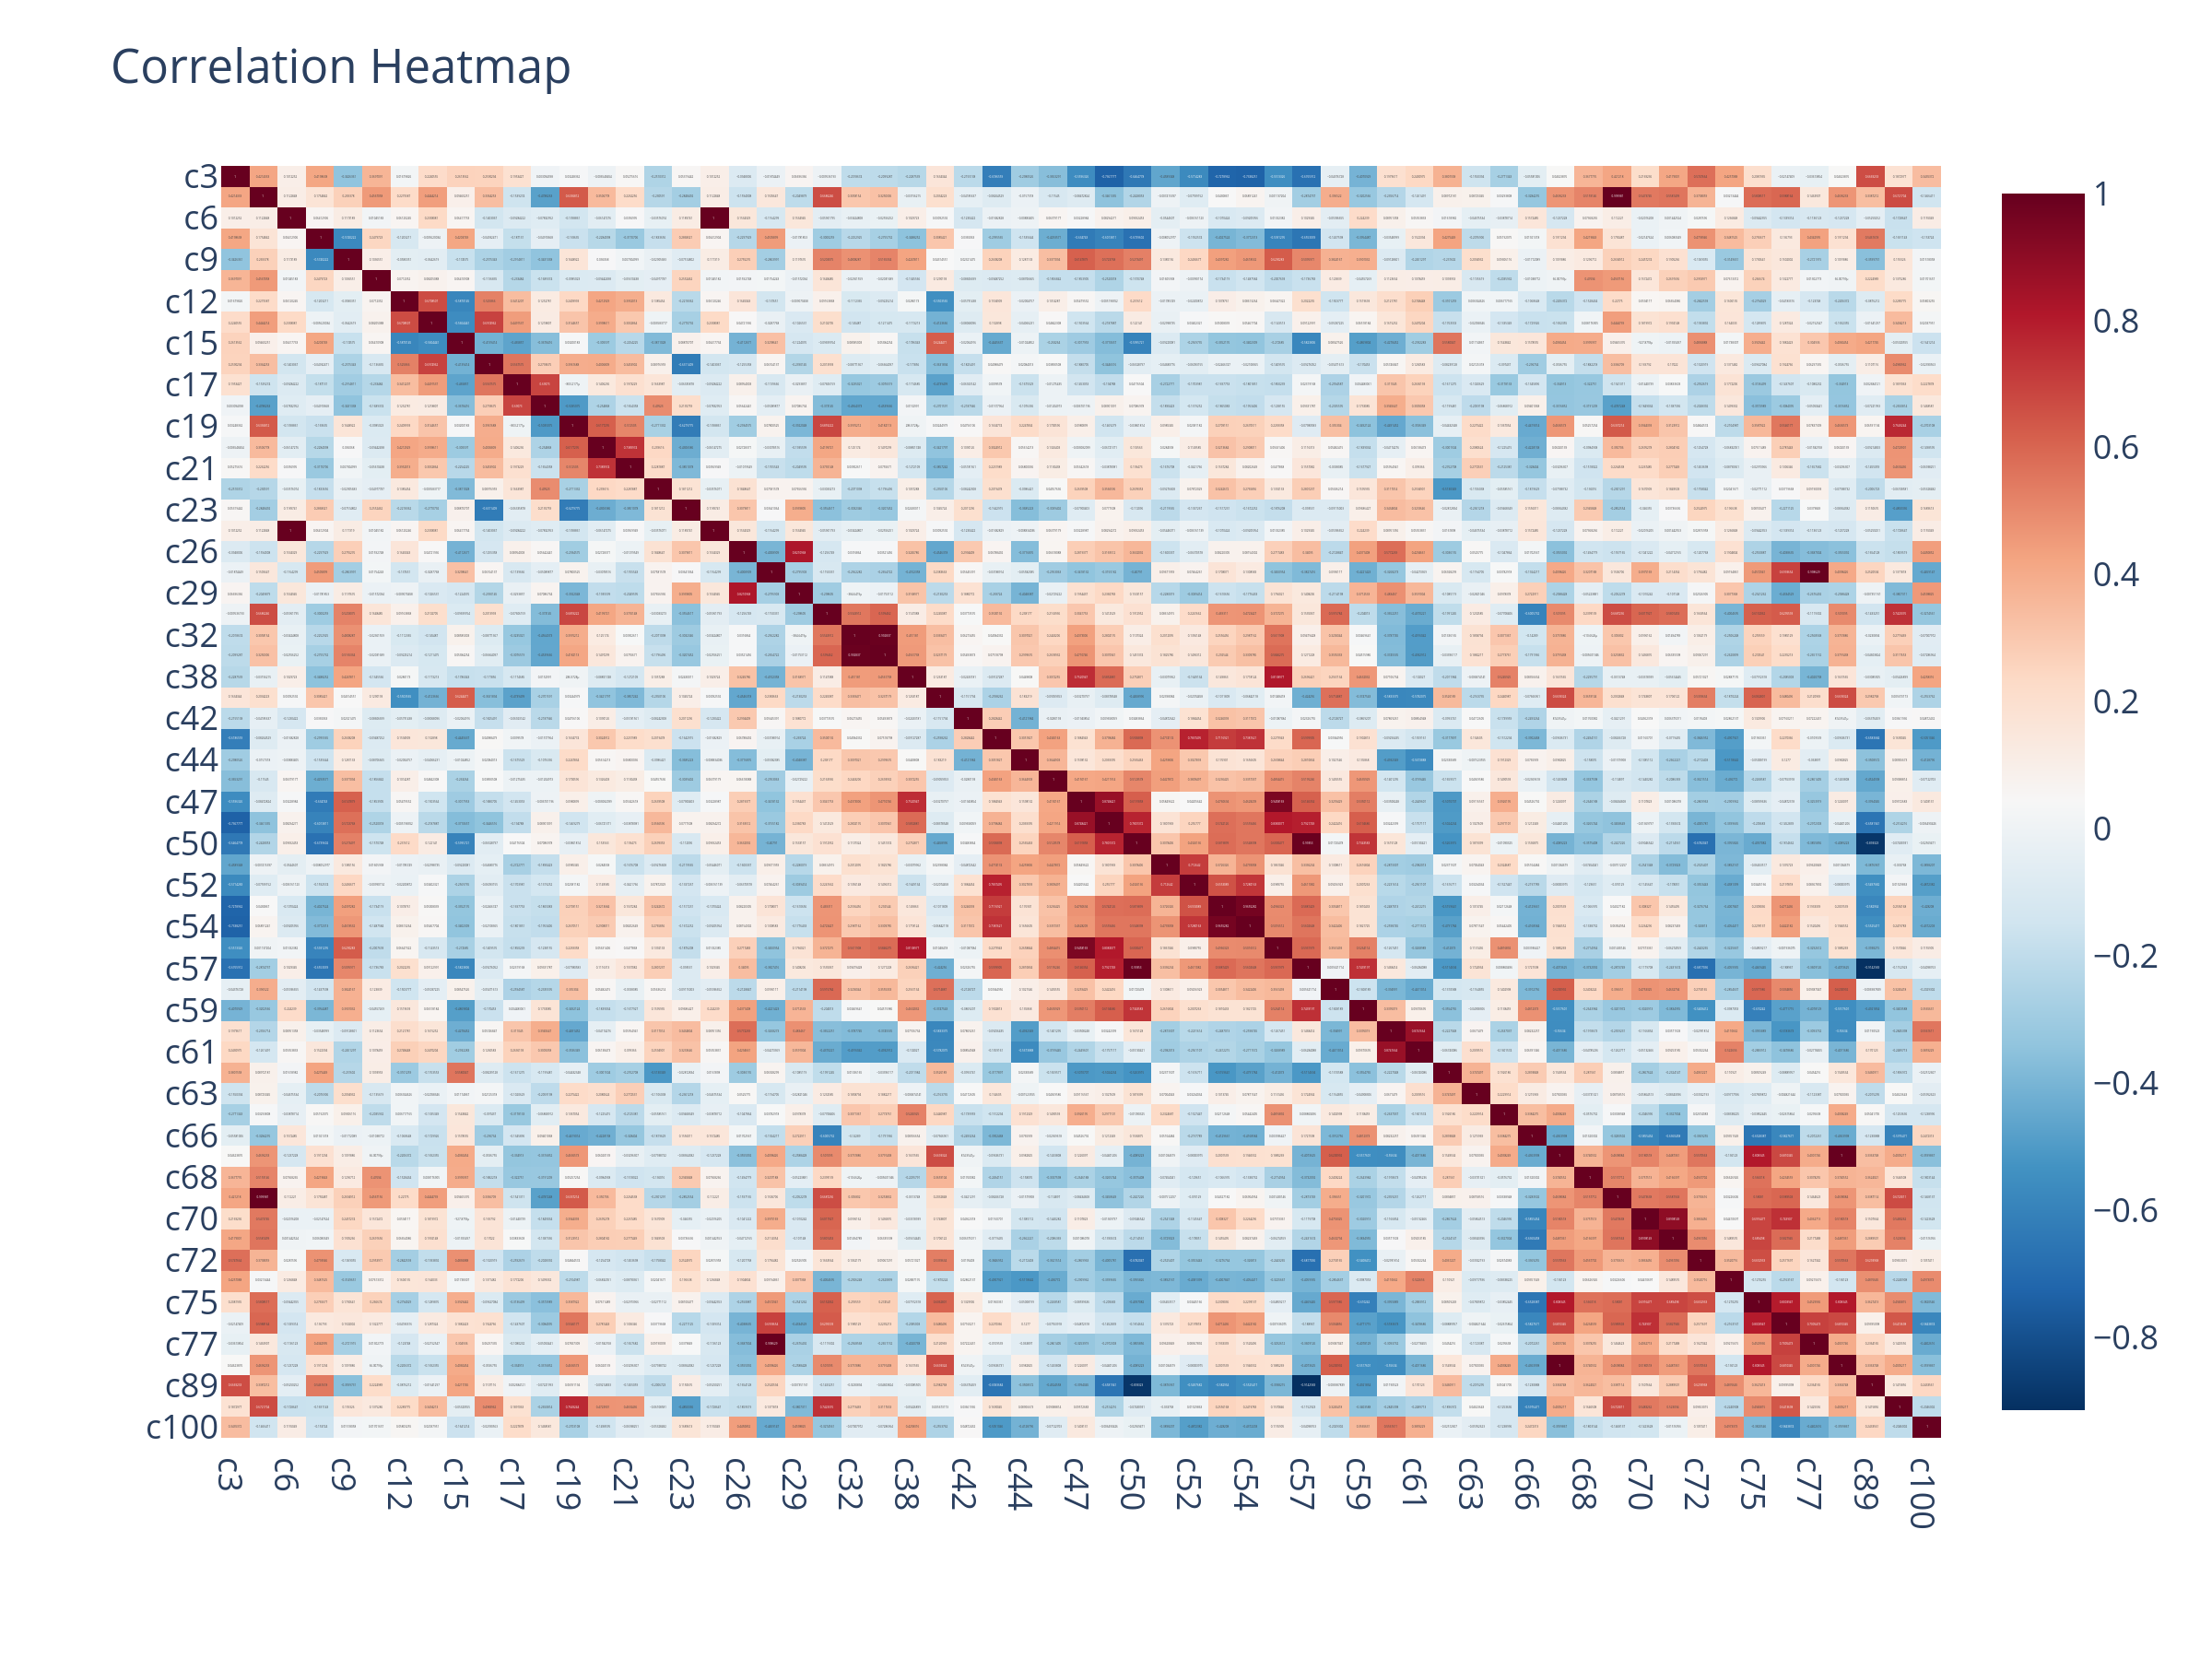
\includegraphics[width=0.6\textwidth]{Images/correlation_heatmap.png}
    \caption{Correlation Heatmap}
\end{figure}


\subsubsection{Multicollinearity Assessment}
Variance Inflation Factor (VIF) was calculated to identify multicollinearity among features.

\begin{lstlisting}[language=Python]
from statsmodels.stats.outliers_influence import variance_inflation_factor

vif_data = pd.DataFrame()
vif_data["feature"] = df_scaled.columns
vif_data["VIF"] = [variance_inflation_factor(df_scaled.values, i) for i in range(len(df_scaled.columns))]
print(vif_data)
\end{lstlisting}

\subsubsection{Dealing with Correlated Columns}
Based on the correlation and VIF analysis, columns with high correlation (greater than 0.8) or high VIF values (greater than 10) were identified and removed.

\begin{lstlisting}[language=Python]
# Dropping correlated columns based on threshold
corr_threshold = 0.8
columns_to_drop = set()

for i in range(len(corr_matrix.columns)):
    for j in range(i):
        if abs(corr_matrix.iloc[i, j]) > corr_threshold:
            colname = corr_matrix.columns[i]
            columns_to_drop.add(colname)

df_scaled.drop(columns=columns_to_drop, inplace=True)
\end{lstlisting}

\subsubsection{Principal Component Analysis (PCA)}
PCA was conducted to reduce the dimensionality of the dataset, both before and after addressing multicollinearity. Elbow diagrams were generated to visualize cumulative explained variance.

\begin{lstlisting}[language=Python]
from sklearn.decomposition import PCA

# PCA before removing correlated features
pca_initial = PCA()
df_pca_initial = pca_initial.fit_transform(df_scaled)
explained_variance_initial = pca_initial.explained_variance_ratio_

# PCA after removing correlated features
pca_final = PCA()
df_pca_final = pca_final.fit_transform(df_scaled)
explained_variance_final = pca_final.explained_variance_ratio_

# Cumulative explained variance
cumulative_variance_initial = np.cumsum(explained_variance_initial)
cumulative_variance_final = np.cumsum(explained_variance_final)
\end{lstlisting}

\subsubsection{Elbow Diagram Creation}
Elbow diagrams were plotted to visualize the explained variance.

\begin{lstlisting}[language=Python]
# Elbow Diagram before removing correlated features
plt.figure(figsize=(12, 6))
plt.plot(range(1, len(cumulative_variance_initial) + 1), cumulative_variance_initial, marker='o')
plt.title('Elbow Diagram (Before Removing Correlated Features)')
plt.xlabel('Number of Components')
plt.ylabel('Cumulative Explained Variance')
plt.grid()
plt.show()

# Elbow Diagram after removing correlated features
plt.figure(figsize=(12, 6))
plt.plot(range(1, len(cumulative_variance_final) + 1), cumulative_variance_final, marker='o', color='orange')
plt.title('Elbow Diagram (After Removing Correlated Features)')
plt.xlabel('Number of Components')
plt.ylabel('Cumulative Explained Variance')
plt.grid()
plt.show()
\end{lstlisting}

\subsection{Results}

\subsubsection{Data Cleaning Results}
The cleaning process resulted in the removal of columns with low variance and handling of missing values. The number of columns dropped due to low variance was \texttt{len(low\_variance\_columns)}.

\subsubsection{Correlation Analysis Results}
The correlation heatmap indicated the presence of highly correlated features. A total of \texttt{len(columns\_to\_drop)} columns were dropped due to high correlation.

% \subsubsection{VIF Analysis Results}
% The VIF analysis showed the following features with high VIF values:
% \begin{center}
% \begin{tabular}{l c}
% \toprule
% Feature & VIF \\
% \midrule
% % Insert VIF results here
% \bottomrule
% \end{tabular}
% \end{center}

\subsubsection{PCA Results}
The PCA results showed that the optimal number of components explaining at least 95\% of the variance was determined. The cumulative variance explained for the initial and final PCA were \texttt{explained\_variance\_initial} and \texttt{explained\_variance\_final} respectively.

\begin{figure}[H]
    \centering
    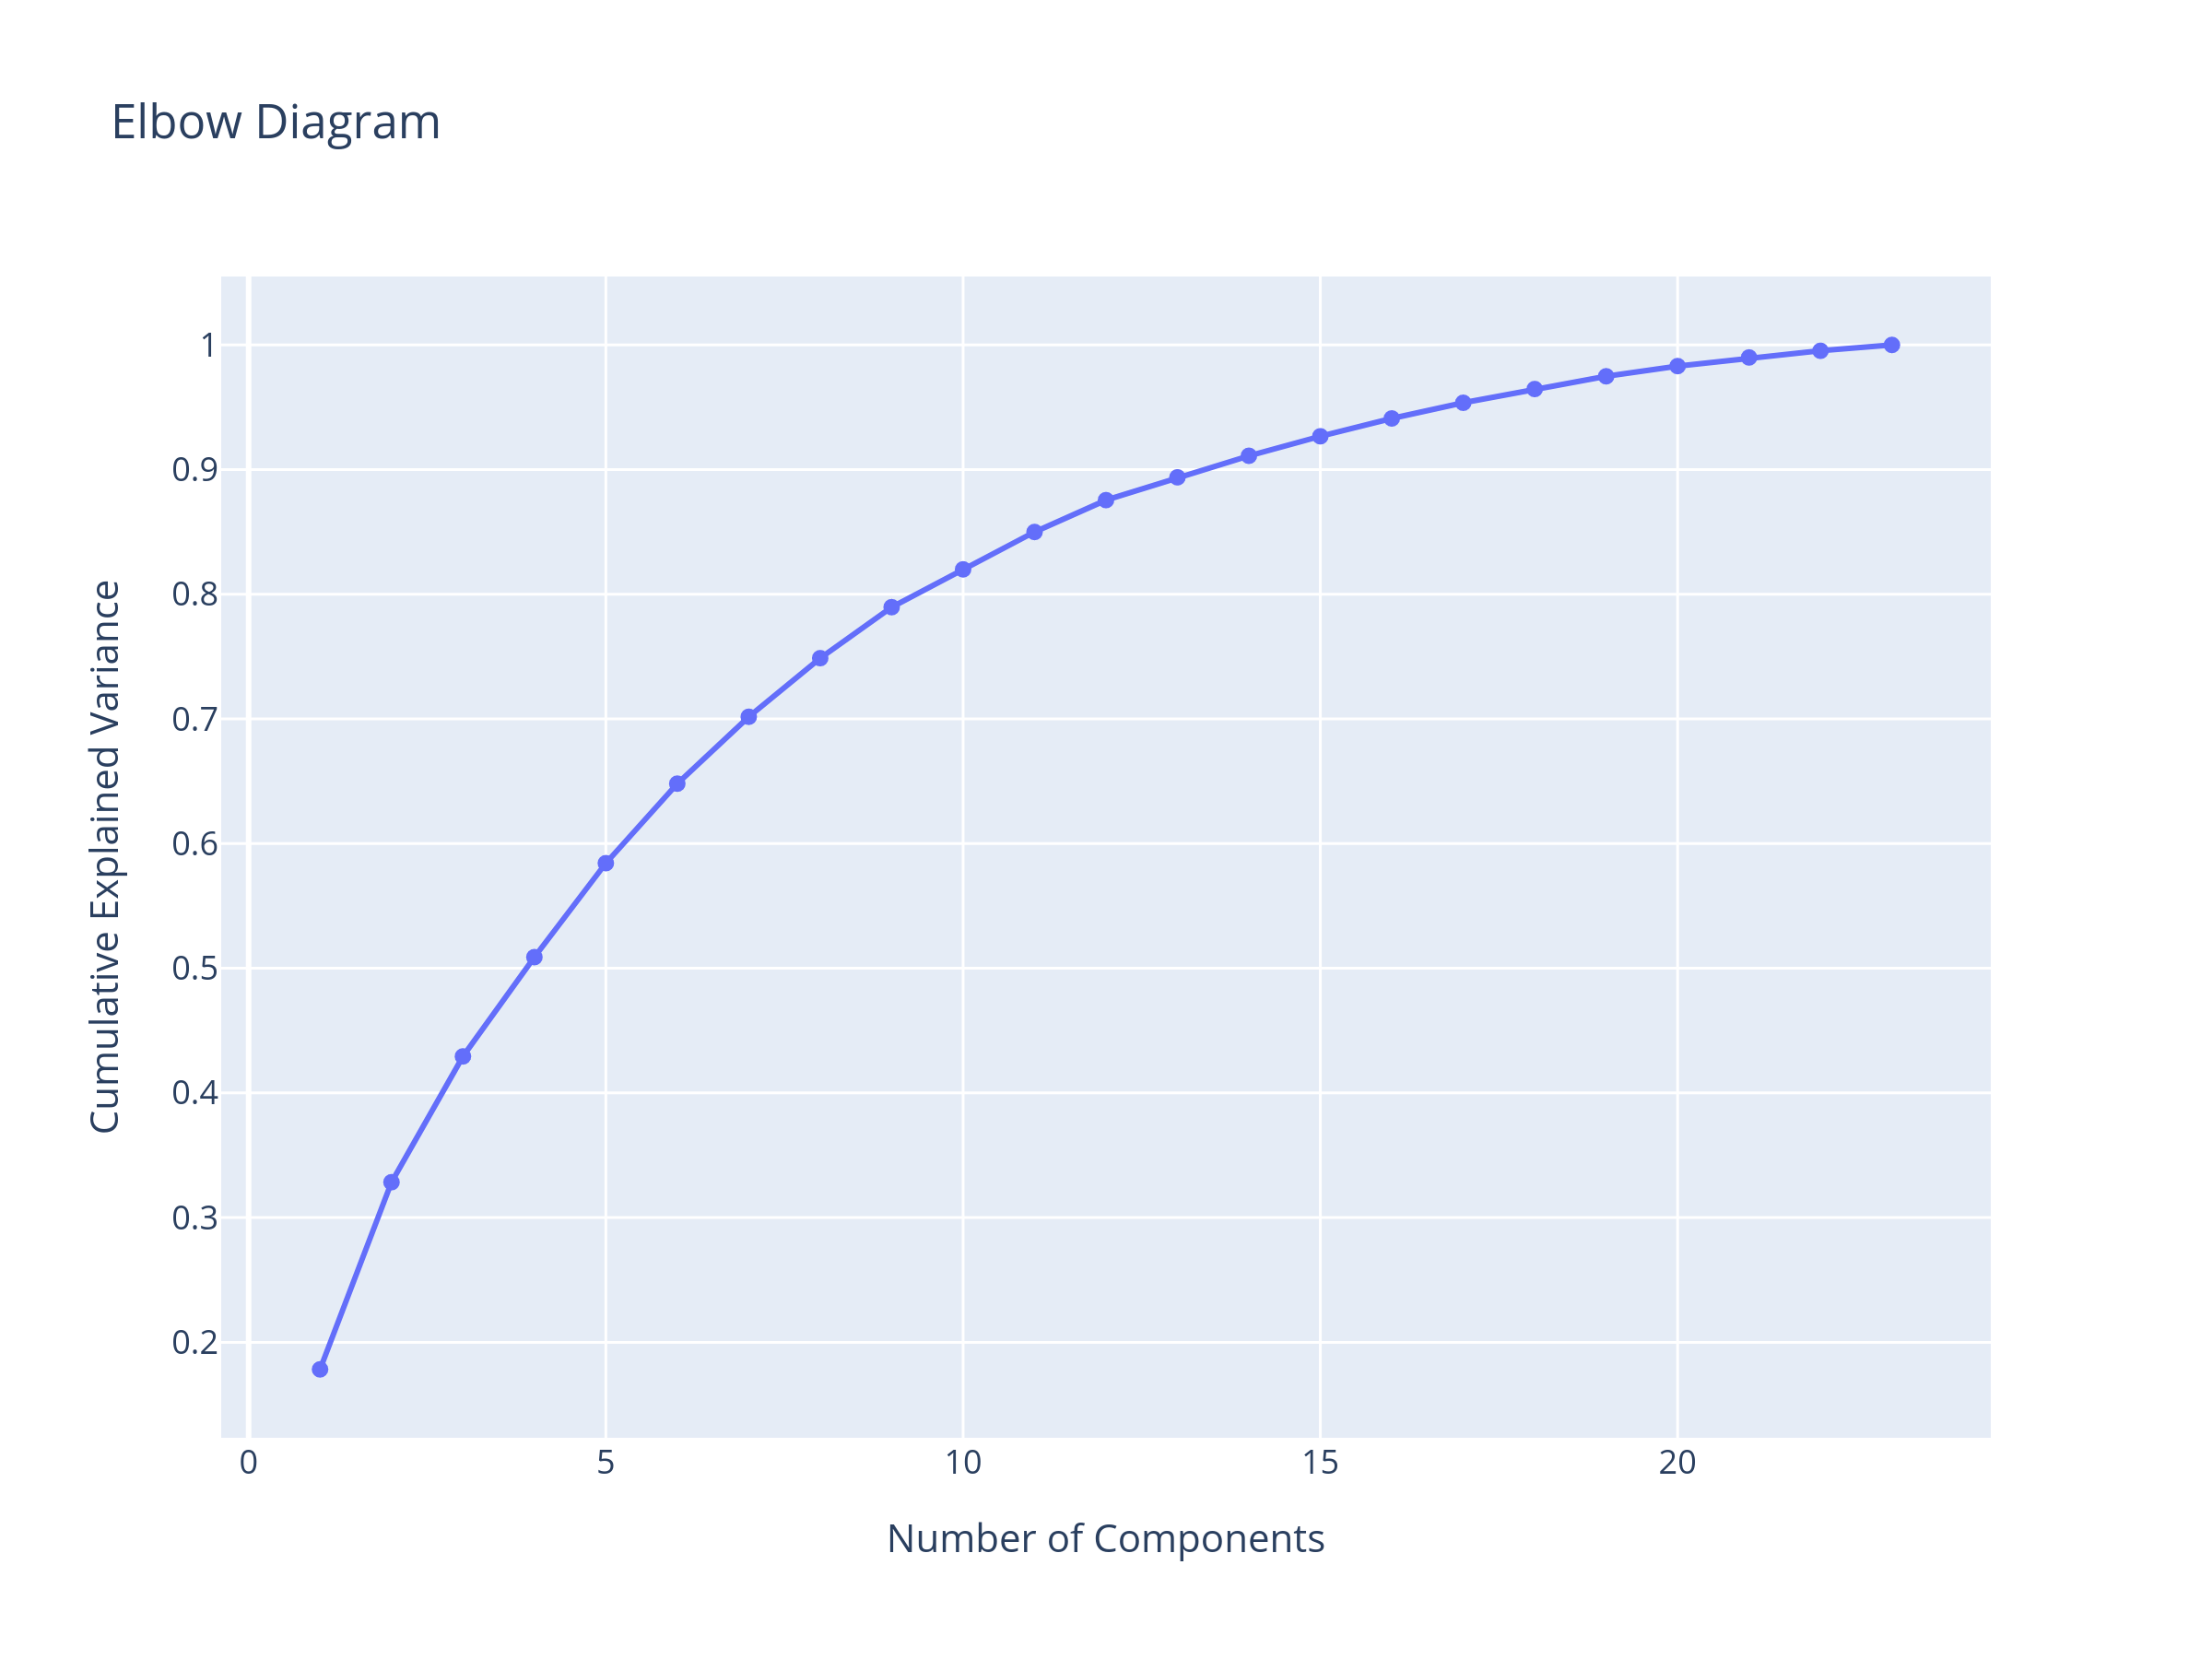
\includegraphics[width=0.6\textwidth]{Images/elbow_diagram_before_vif.png}
    \caption{Elbow Diagram (Before Removing Correlated Features)}
\end{figure}

\begin{figure}[H]
    \centering
    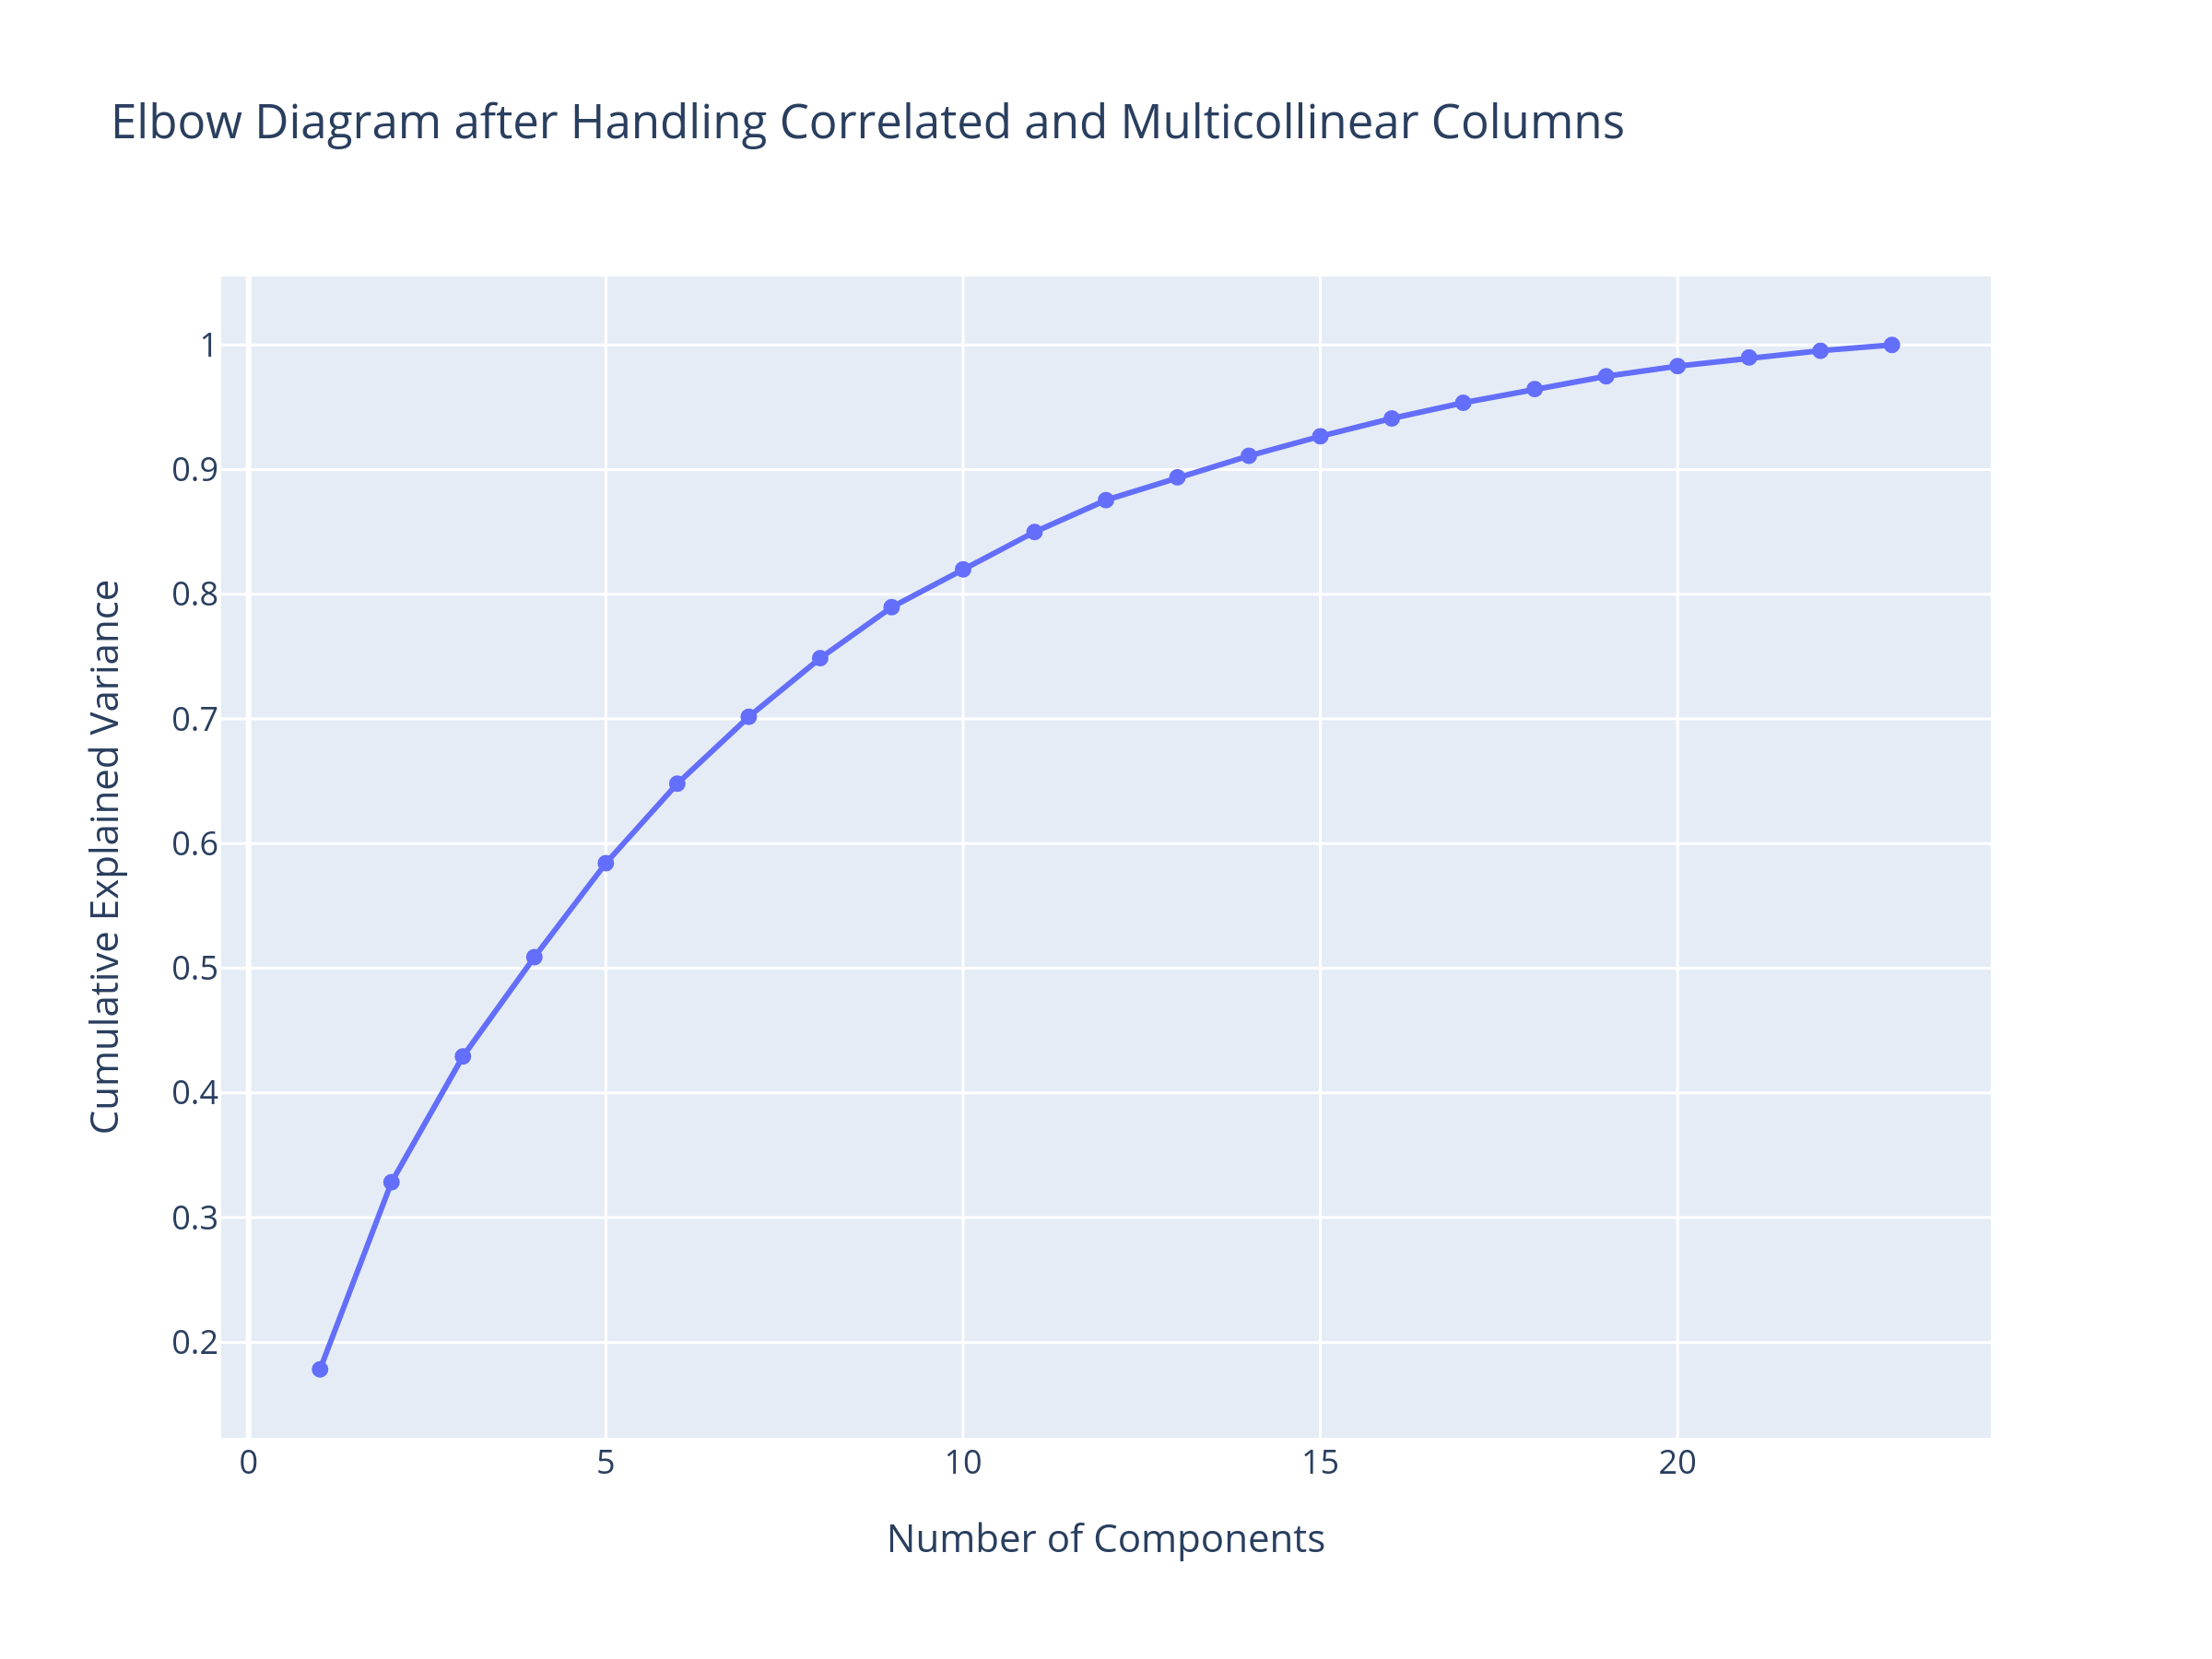
\includegraphics[width=0.6\textwidth]{Images/elbow_diagram_after_vif.png}
    \caption{Elbow Diagram (After Removing Correlated Features)}
\end{figure}

\subsection{Conclusion}
This analysis provided insights into the dataset, with significant findings related to data cleaning, correlation, multicollinearity, and dimensionality reduction through PCA. The methodology applied can be used as a standard approach for similar datasets.

\clearpage
\section{Problem 3}

\subsection{Introduction}
This report details the implementation of dimensionality reduction techniques using Principal Component Analysis (PCA) and t-distributed Stochastic Neighbor Embedding (t-SNE) on the MNIST dataset and another dataset referred to as the e6 dataset. These techniques are crucial in exploratory data analysis, especially in high-dimensional datasets, allowing for better visualization and interpretation.

\subsection{Data Loading and Preprocessing}
The code begins by loading the MNIST test dataset and the e6 dataset. For the MNIST dataset, the features are separated from the labels. The e6 dataset undergoes additional preprocessing steps to handle missing values and convert date formats.

\subsubsection{Loading the MNIST Dataset}
The following code snippet loads the MNIST dataset:
\begin{lstlisting}[language=Python]
mnist_test = pd.read_csv('mnist_test.csv')
X = mnist_test.drop('label', axis=1)
y = mnist_test['label']
\end{lstlisting}

\subsubsection{Loading the e6 Dataset}
The e6 dataset is loaded and preprocessed to manage missing values and convert the datetime column:
\begin{lstlisting}[language=Python]
e6_data = pd.read_csv('e6-Run2-June22-subset-100-cols.csv')
e6_data.replace('#REF!', np.nan, inplace=True)
e6_data.iloc[:, 0] = pd.to_datetime(e6_data.iloc[:, 0], format='%d-%m-%Y')
\end{lstlisting}

\subsection{Standardization}
Standardization is a critical step in data preprocessing to ensure that each feature contributes equally to the analysis. This is achieved using the \texttt{StandardScaler} class from the \texttt{sklearn.preprocessing} module.

\begin{lstlisting}[language=Python]
scaler = StandardScaler()
X_scaled = scaler.fit_transform(X)
\end{lstlisting}

\subsection{Dimensionality Reduction}
Two dimensionality reduction techniques are applied to the datasets: PCA and t-SNE.

\subsubsection{PCA Implementation}
PCA is used to reduce the dimensionality of the MNIST dataset while analyzing the explained variance. The cumulative explained variance is computed and visualized to identify the optimal number of components.

\begin{lstlisting}[language=Python]
pca = PCA()
X_pca = pca.fit_transform(X_scaled)
explained_variance_ratio = pca.explained_variance_ratio_
cumulative_variance = np.cumsum(explained_variance_ratio)
\end{lstlisting}

The elbow diagram illustrating the cumulative explained variance is shown in Figure \ref{fig:elbow_diagram}.

\begin{figure}[H]
    \centering
    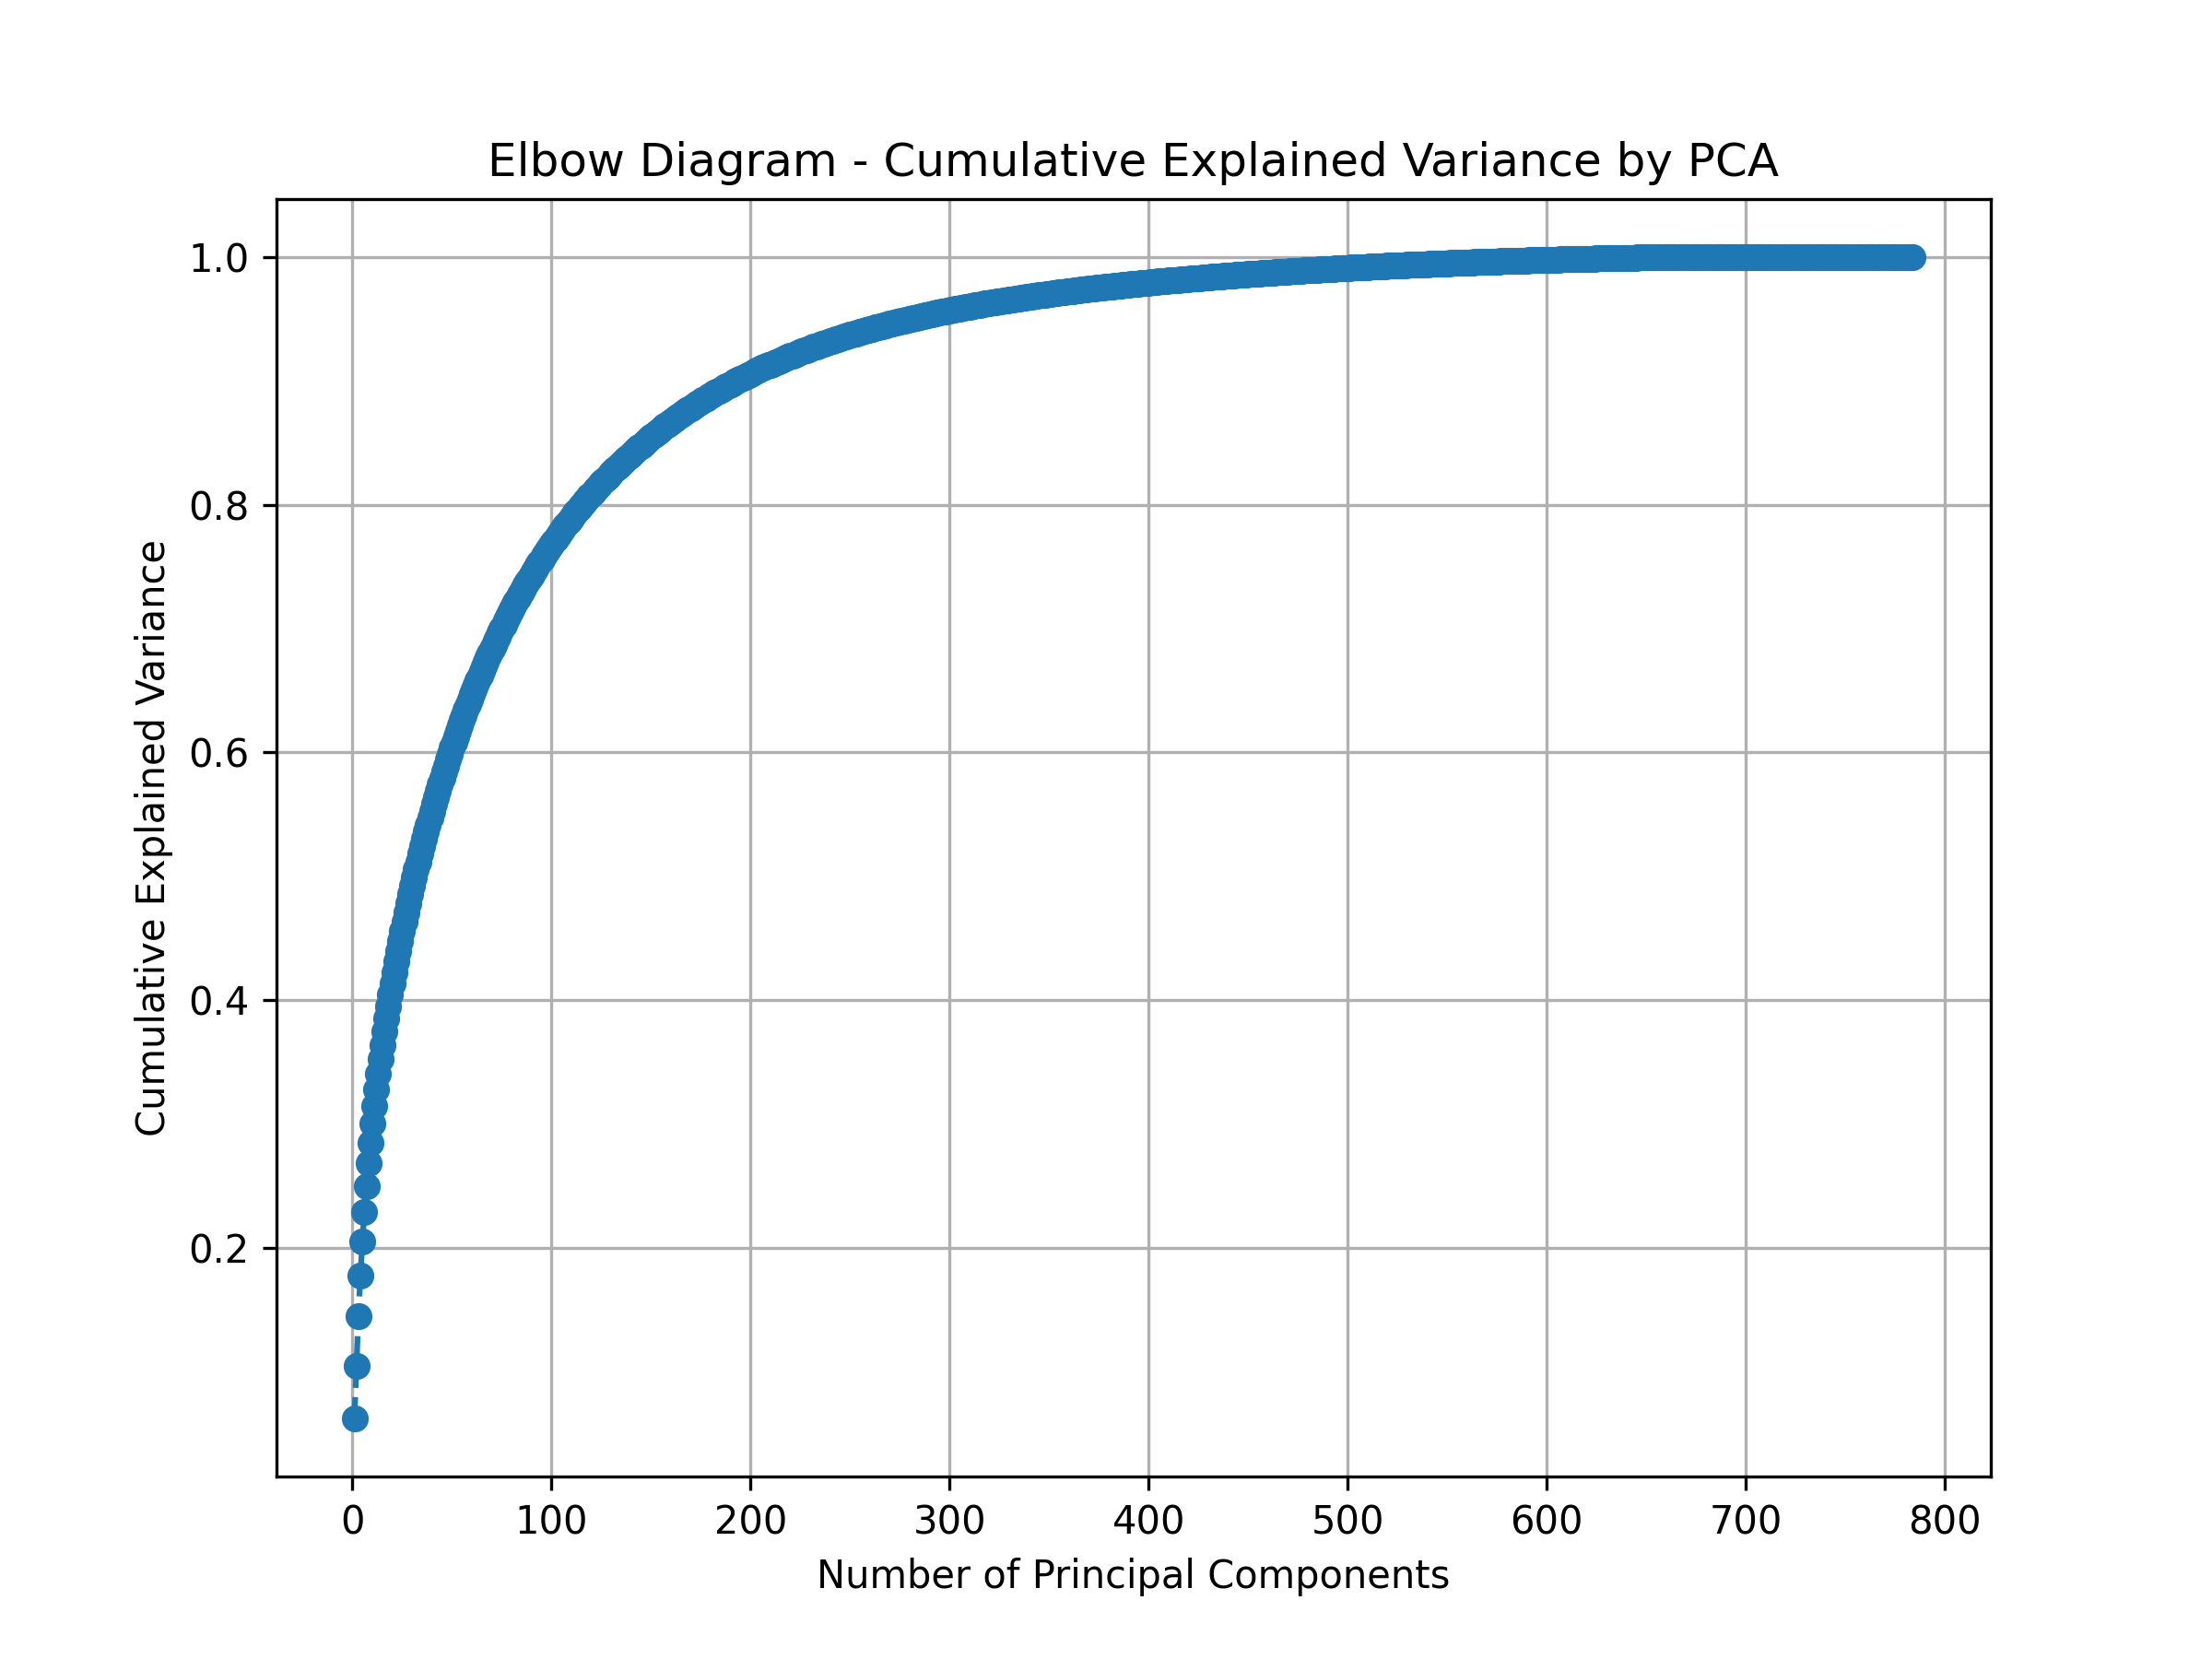
\includegraphics[width=0.6\textwidth]{Images/P3-elbow_diagram.png}
    \caption{Elbow Diagram - Cumulative Explained Variance by PCA}
    \label{fig:elbow_diagram}
\end{figure}

The first two principal components are visualized in the scatter plot in Figure \ref{fig:pca_scatter_plot}.

\begin{figure}[H]
    \centering
    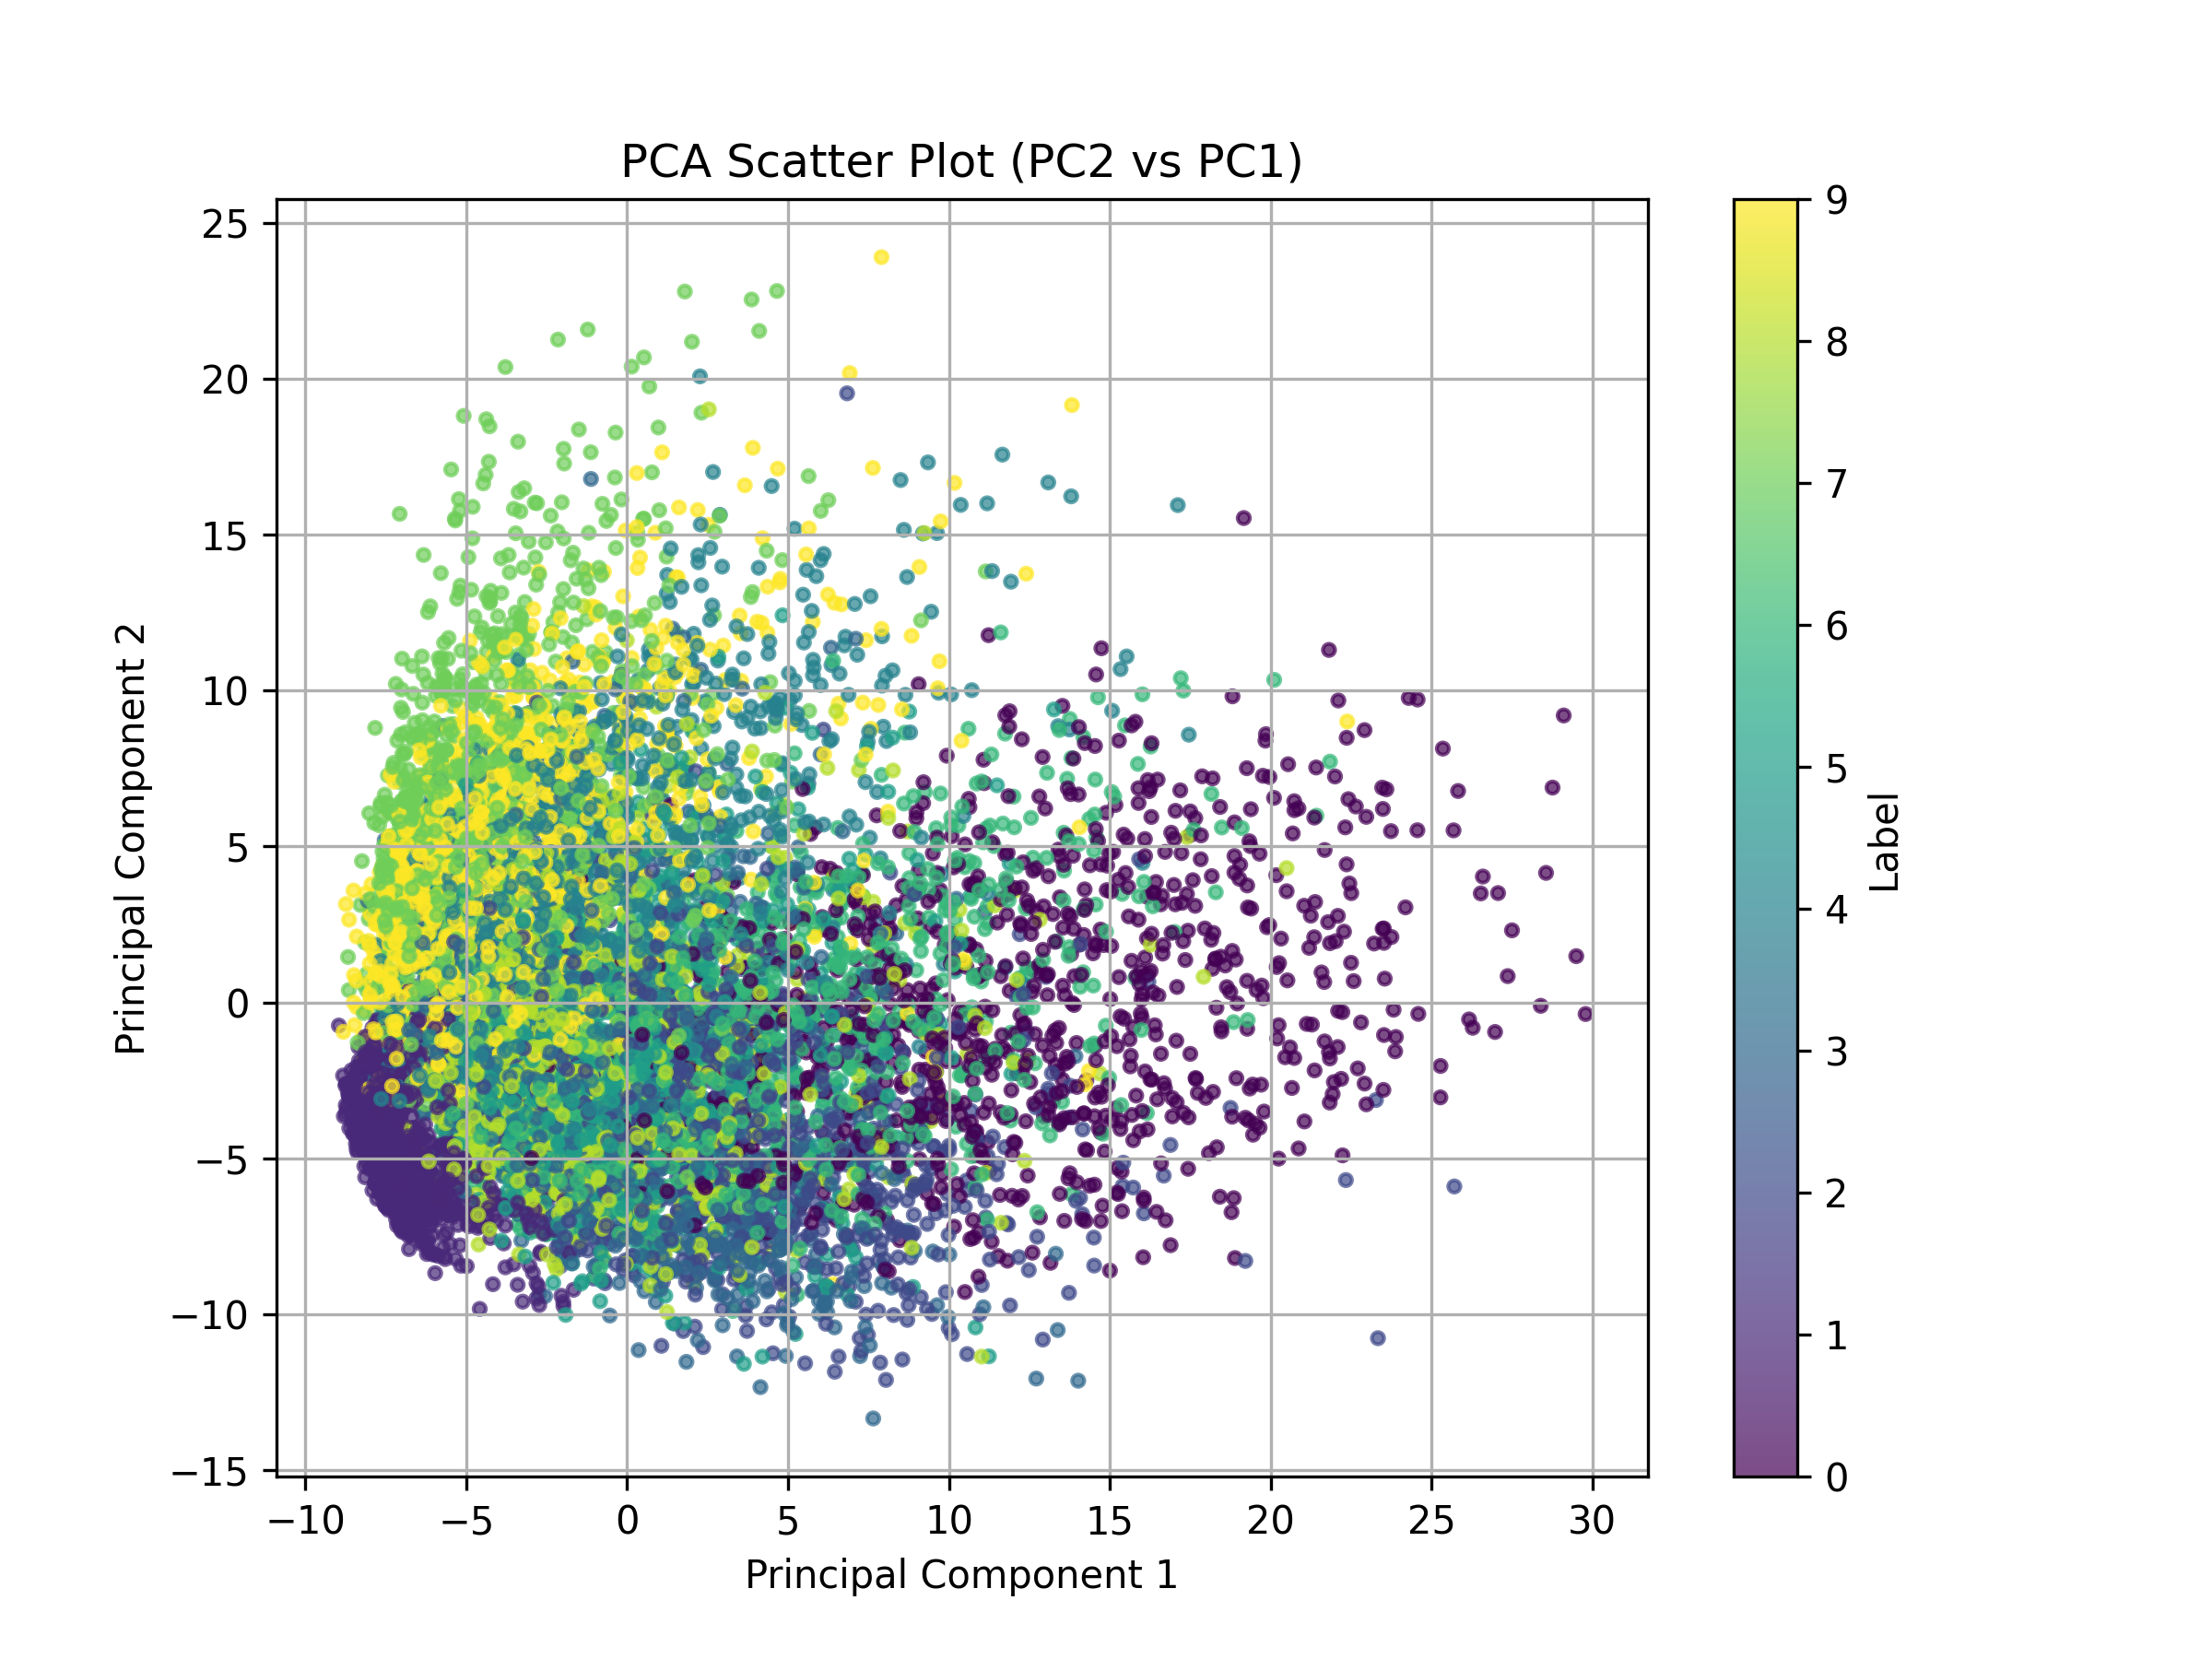
\includegraphics[width=0.6\textwidth]{Images/P3-pca_scatter_plot.png}
    \caption{PCA Scatter Plot (PC2 vs PC1)}
    \label{fig:pca_scatter_plot}
\end{figure}

\subsubsection{t-SNE Implementation}
t-SNE is applied to visualize the high-dimensional MNIST dataset in two dimensions. The following code snippet demonstrates this process:

\begin{lstlisting}[language=Python]
tsne = TSNE(n_components=2, random_state=42)
X_tsne = tsne.fit_transform(X_scaled)
\end{lstlisting}

The t-SNE scatter plot is shown in Figure \ref{fig:tsne_scatter_plot}.

\begin{figure}[H]
    \centering
    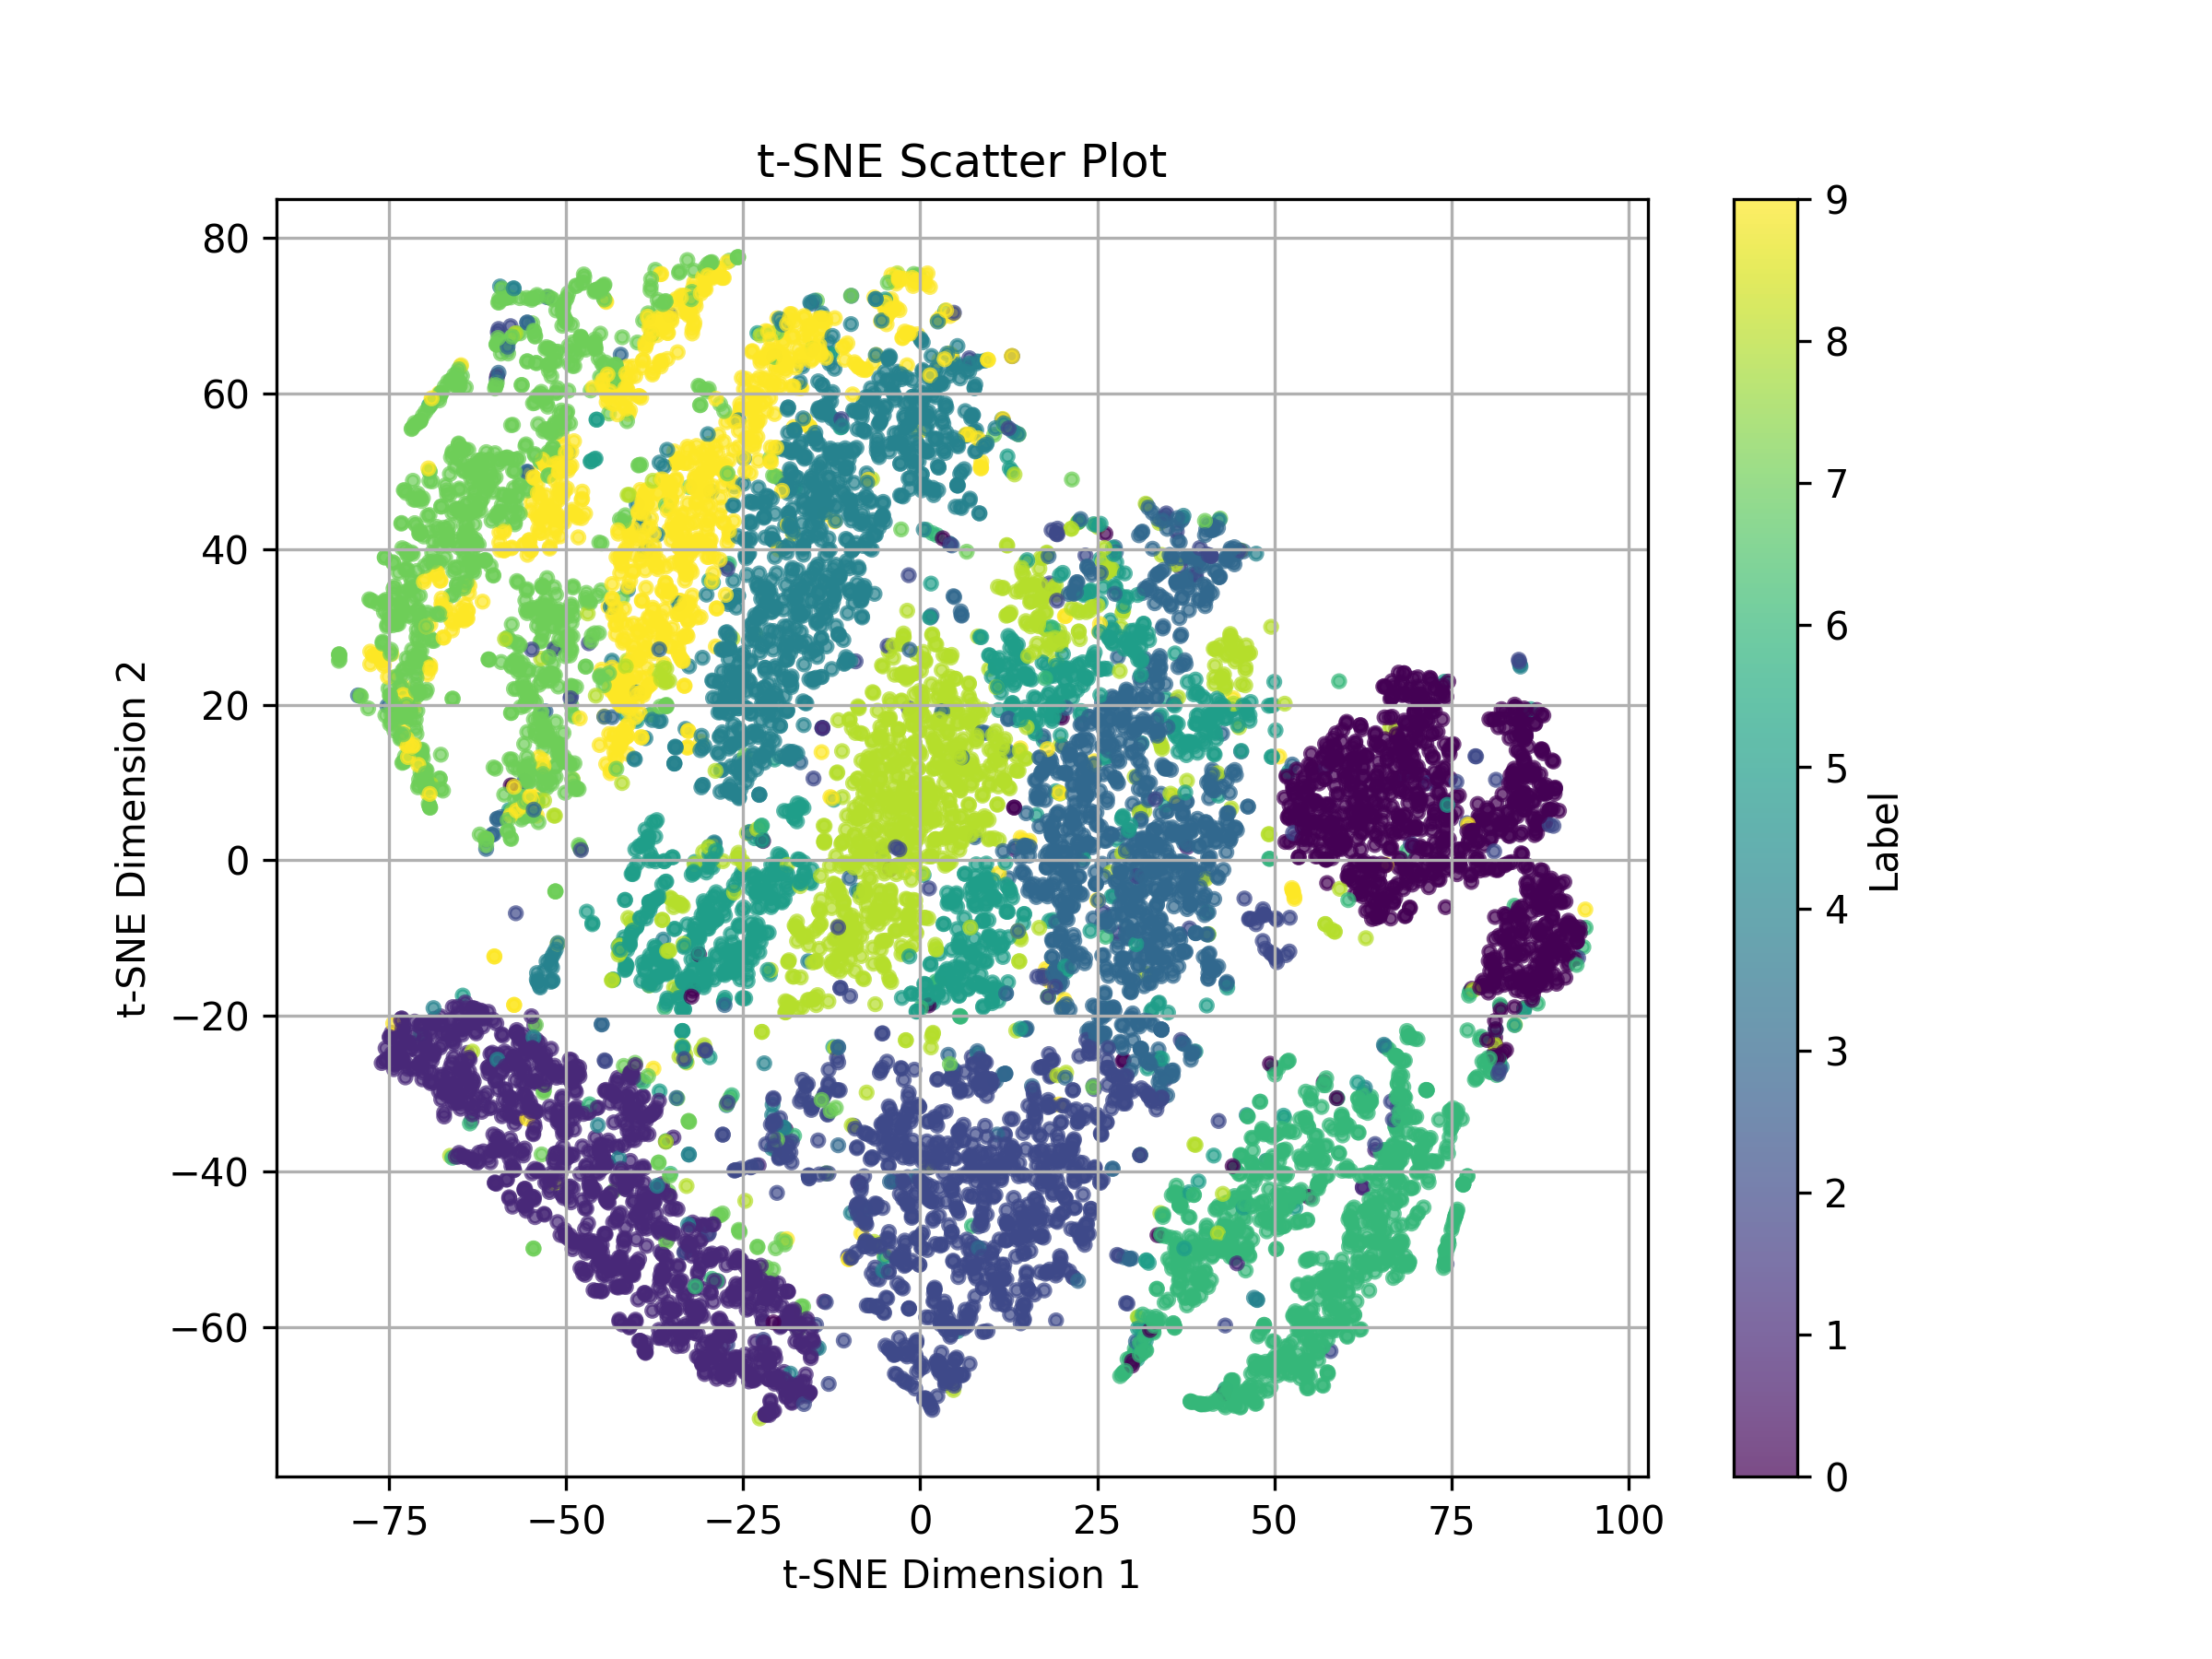
\includegraphics[width=0.6\textwidth]{Images/P3-tsne_scatter_plot.png}
    \caption{t-SNE Scatter Plot for MNIST Dataset}
    \label{fig:tsne_scatter_plot}
\end{figure}

Similarly, t-SNE is applied to the e6 dataset, and the resulting scatter plot is shown in Figure \ref{fig:tsne_scatter_plot_e6}.

\begin{figure}[H]
    \centering
    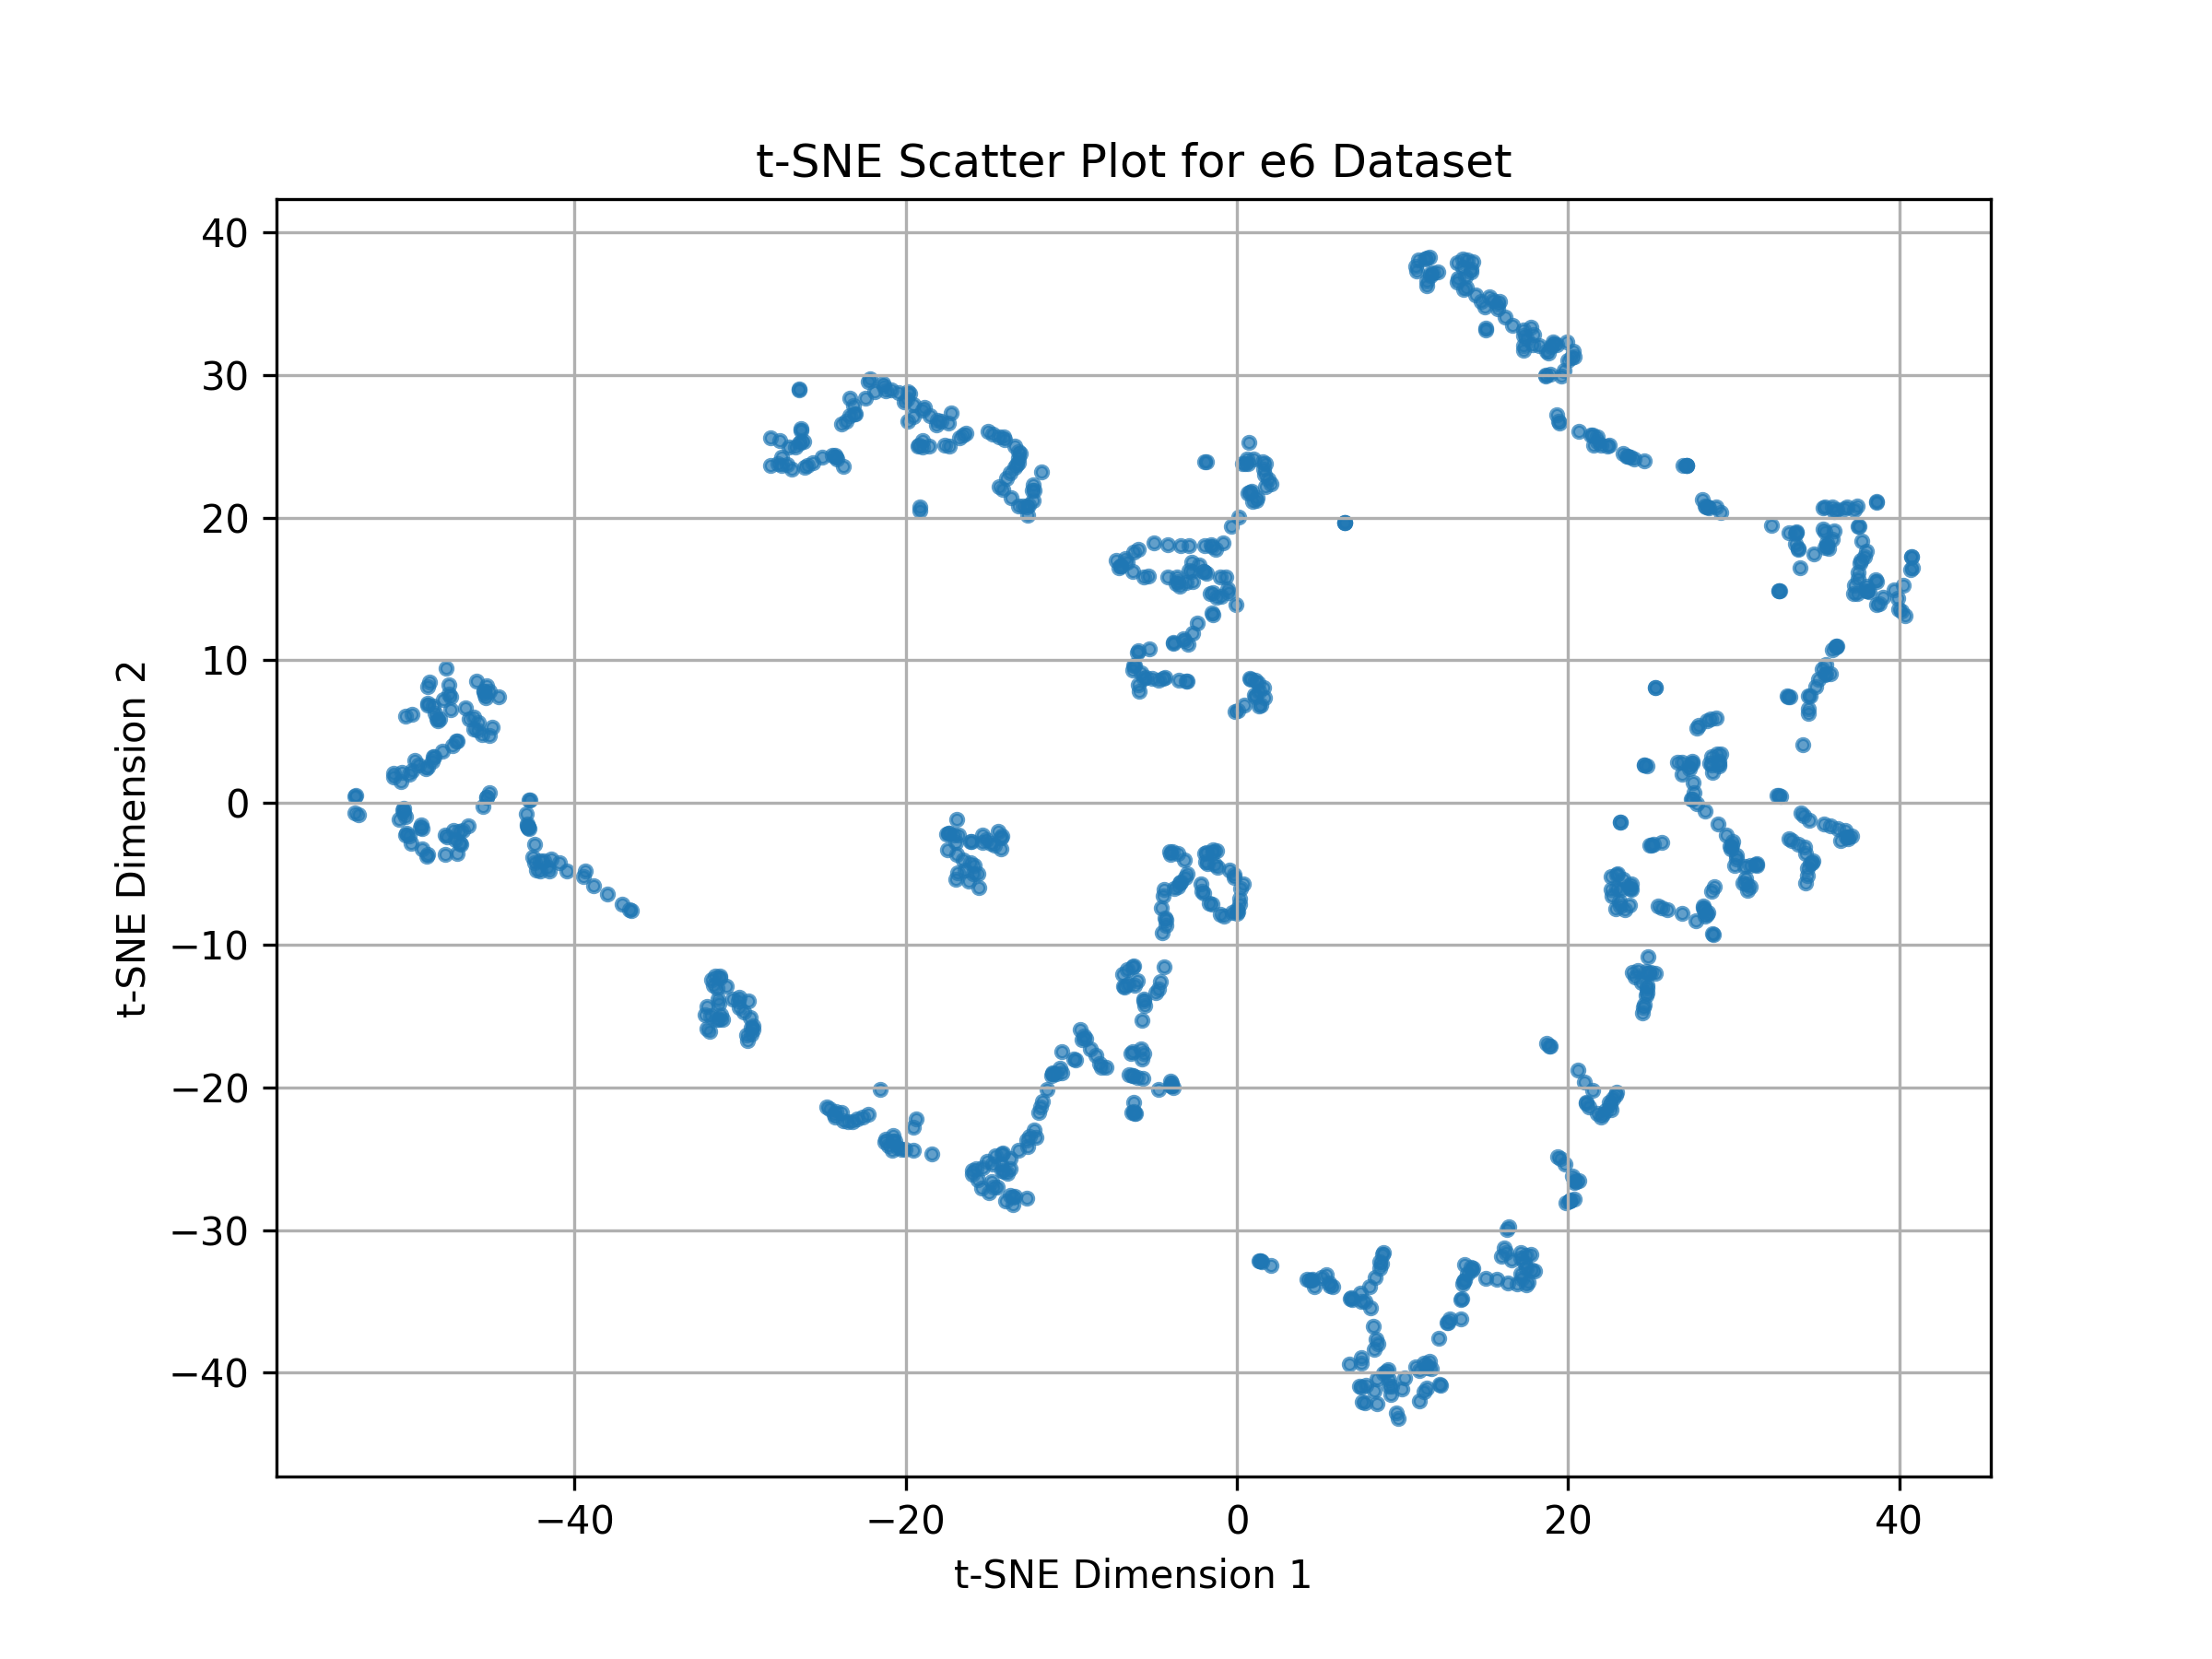
\includegraphics[width=0.8\textwidth]{Images/P3-tsne_scatter_plot_e6.png}
    \caption{t-SNE Scatter Plot for e6 Dataset}
    \label{fig:tsne_scatter_plot_e6}
\end{figure}

\subsection{Analysis and Insights}
The elbow diagram allows us to determine the optimal number of principal components for PCA by identifying the 'elbow' point, which indicates a suitable number of components to retain while preserving variance. The scatter plots provide visual insights into the distribution of the data, helping to identify clusters and separations between different classes.

PCA effectively retains the global structure of the data, while t-SNE emphasizes local similarities, making it particularly useful for classification problems in high-dimensional datasets.

\subsection{Conclusion}
This report demonstrates the effective application of PCA and t-SNE for dimensionality reduction and visualization of the MNIST and e6 datasets. The combination of PCA's explained variance analysis and t-SNE's visualization capabilities provides a comprehensive view of the inherent structures in the datasets, making it a valuable approach in exploratory data analysis and machine learning preprocessing workflows.

\section{Introduction}
This report summarizes the learnings from three Python scripts that involve data analysis, data cleaning, and machine learning techniques. The scripts demonstrate various methodologies for exploring, processing, and visualizing data to extract meaningful insights.

\subsection{Problem 1: Analyzing HT R Phase Current Data}
The first script focuses on analyzing a dataset containing the HT R Phase Current over time. The key tasks and learnings from this analysis are as follows:

\subsubsection{Exploratory Data Analysis (EDA)}
The initial step involved loading the data and performing descriptive statistics to understand the dataset better. The \texttt{describe()} method provided an overview of the data distribution, highlighting key metrics such as mean, median, and standard deviation.

\subsubsection{Visualization of Current over Time}
Using \texttt{Plotly}, the script visualized the HT R Phase Current over time, allowing for a dynamic representation of trends and anomalies. This visualization is crucial for identifying periods of instability.

\subsubsection{Identifying Unstable Periods}
A specific two-week period (July 30, 2019, to August 14, 2019) was identified as unstable. The script plotted the current values during this period to visualize fluctuations.

\subsubsection{Outlier Handling and Data Imputation}
Various methods were applied to handle outliers and missing data:
\begin{itemize}
    \item \textbf{Imputation:} Replacing outliers with the mean or median values.
    \item \textbf{Trimming:} Removing outliers based on the 10th and 90th percentiles.
    \item \textbf{Capping:} Setting maximum and minimum thresholds for current values.
    \item \textbf{Robust Estimation:} Using RANSAC regression to estimate current values while ignoring outliers.
    \item \textbf{Loess Smoothing:} Applying local regression to identify trends in the data.
\end{itemize}

\subsubsection{Visualization of Processed Data}
The script generated several plots to visualize the original and processed data, demonstrating the impact of different outlier handling methods. This included comparisons of the original data with mean and median imputed data, trimmed data, capped data, robust estimations, and Loess smoothed data.

\subsection{Problem 2: Data Cleaning and Feature Selection}
The second script focuses on data cleaning and feature selection techniques applied to a dataset with 100 columns. The key tasks and learnings from this analysis are as follows:

\subsubsection{Data Loading and Initial Exploration}
Data was loaded from a CSV file, followed by initial explorations such as checking for null values and obtaining summary statistics.

\subsubsection{Handling Low Variance Columns}
Columns with low variance (less than 0.05) were identified and removed, as they provide little useful information for predictive modeling.

\subsubsection{Missing Value Imputation}
Missing values in numeric columns were replaced with the mean of those columns, ensuring that the dataset remains usable for further analysis.

\subsubsection{Outlier Detection and Removal}
Outliers were detected using the Interquartile Range (IQR) method. Rows containing outliers were removed to improve the quality of the dataset.

\subsubsection{Normalization and Standardization}
The numeric data was standardized using \texttt{StandardScaler} from \texttt{sklearn}, allowing for the normalization of features across different scales, which is essential for machine learning algorithms.

\subsubsection{Correlation Analysis}
A correlation heatmap was generated to visualize relationships between features. Highly correlated features (with a threshold of 0.8) were identified, and one feature from each pair was dropped to reduce multicollinearity.

\subsection{Problem 3: Dimensionality Reduction with PCA and t-SNE}
The third script focuses on applying dimensionality reduction techniques, specifically PCA (Principal Component Analysis) and t-SNE (t-distributed Stochastic Neighbor Embedding), to the MNIST dataset and another dataset named E6. The key tasks and learnings from this analysis are as follows:

\subsubsection{PCA Analysis on MNIST}
The script begins by loading the MNIST test dataset and separating features from labels. Key steps in the PCA analysis include:
\begin{itemize}
    \item \textbf{Standardization:} The features were standardized using \texttt{StandardScaler} to ensure that each feature contributes equally to the analysis.
    \item \textbf{PCA Application:} PCA was applied to the standardized data, transforming it into a lower-dimensional space. The explained variance ratio and cumulative variance were calculated to determine the effectiveness of the principal components.
    \item \textbf{Elbow Diagram:} An elbow diagram was created to visualize cumulative explained variance by the number of principal components, helping identify an optimal number of components.
    \item \textbf{Scatter Plot:} A scatter plot was generated to visualize the first two principal components, revealing the distribution of the data in the reduced space.
\end{itemize}

\subsubsection{t-SNE Analysis on MNIST}
Following the PCA analysis, t-SNE was applied to further reduce the dataset to two dimensions:
\begin{itemize}
    \item \textbf{t-SNE Application:} The script applied t-SNE to the standardized MNIST data to create a 2D representation, which is particularly effective for visualizing high-dimensional data.
    \item \textbf{t-SNE Scatter Plot:} A scatter plot was generated to visualize the clusters formed by different digits in the MNIST dataset, providing insights into the separability of classes.
\end{itemize}

\subsubsection{t-SNE Analysis on E6 Dataset}
The script also applied t-SNE to another dataset named E6:
\begin{itemize}
    \item \textbf{Data Loading and Cleaning:} The E6 dataset was loaded, and preprocessing steps included replacing erroneous values with NaN, converting timestamps, and handling missing values.
    \item \textbf{Feature Scaling:} Features were scaled using \texttt{StandardScaler} before applying t-SNE.
    \item \textbf{t-SNE Visualization:} A t-SNE scatter plot was created for the E6 dataset, allowing visualization of the distribution of the data in two dimensions.
\end{itemize}

\subsection{Conclusion}
The scripts illustrate essential techniques in data analysis and machine learning, including exploratory data analysis, outlier handling, feature selection, and dimensionality reduction. The application of PCA and t-SNE provides valuable insights into the structure of high-dimensional datasets, facilitating effective visualization and understanding of complex data relationships.

% \subsection{References}
% \begin{itemize}
%     \item \texttt{pandas} documentation: \url{https://pandas.pydata.org/pandas-docs/stable/}
%     \item \texttt{numpy} documentation: \url{https://numpy.org/doc/stable/}
%     \item \texttt{scikit-learn} documentation: \url{https://scikit-learn.org/stable/documentation.html}
%     \item \texttt{matplotlib} documentation: \url{https://matplotlib.org/stable/contents.html}
%     \item \texttt{plotly} documentation: \url{https://plotly.com/python/}
% \end{itemize}

\end{document}